\section{Light Attenuation}

Light attenuation was determined by measuring the MIP energy as a function of distance from the readout edge of each U,V,W view.  Fig.~\ref{fig:attendef} shows a schematic of how crossing strips are used to define the hit distance. The overlap of the measured strip and the crossing strip creates a trapezoidal bin formed by the overlap of two different strip orientations. The width of this physical bin is given by
\begin{equation}
    s = \frac{w}{\sin{\alpha}} = \frac{w}{\cos{\beta}}
    \label{eq:s}
\end{equation}
where $w$ is a single scintillator strip width ($\approx 4.5$cm). The strip number is converted into distance using equations \ref{eq:udist}-\ref{eq:wdist},\ref{eq:s}, plus an offset such that the distance is referenced to the center of the physical bin. 

\begin{figure}[h]
\centering
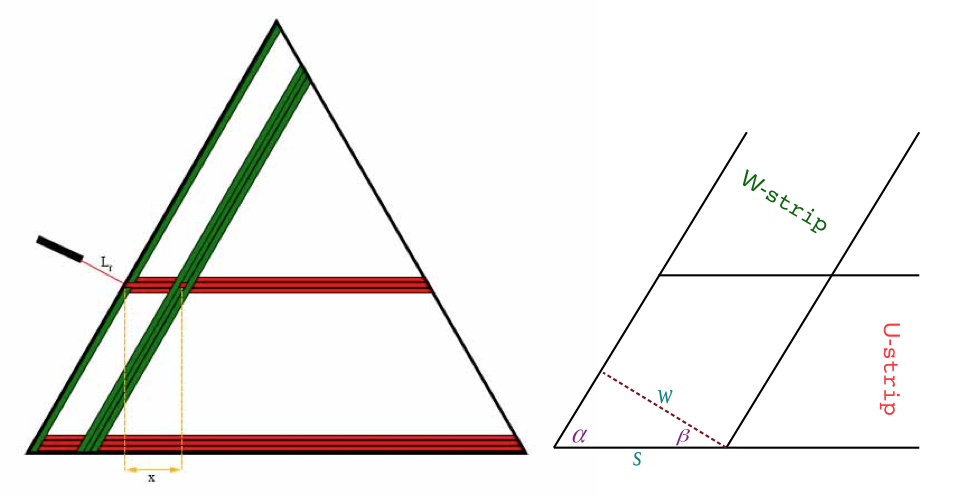
\includegraphics[height= 2in, keepaspectratio = true]{attendef}
\caption{LEFT: Schematic demonstrates the use of crossing strips to measure distance from edge of PCAL triangle. RIGHT: Outline of a generic intersection of a u and w strip. The distance between the trapezoidal
 area and the PCAL edge can be represented by a linear function of $s$.}
\label{fig:attendef}
\end{figure}

Fig.~\ref{fig:adcvdist} shows a 2-D histogram of the measured MIP energy versus the PMT number of the crossing strip.  The data clearly show the decrease in the MIP peak with distance. The next sections describe how the MIP energy for each distance slice is determined, and the fitting function used to describe the attenuation.

\begin{figure}[h]
\centering
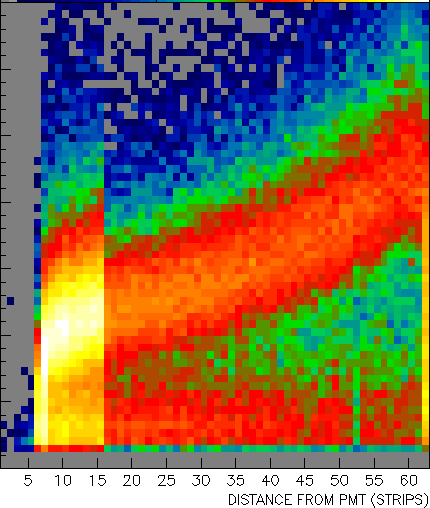
\includegraphics[width= 2.5in, keepaspectratio = true]{adcvdist}
\caption{Cosmic data showing ADC plotted vs crossing strip number.  In this case PMT 62 is closest to the readout end.}
\label{fig:adcvdist}
\end{figure}

\subsection{Fitting to MIP Peaks}
\label{Sec:fitToADCOutput}

Following event selection to isolate single pixel hits, the resulting energy loss distributions show two features:

\begin{enumerate}
\item MIP peak with a mean which is position dependent, corresponding to tracks which pass through all five scintillator layers in the measured pixel.
\item Background which diminishes with increasing pulse height and peaks near the ADC threshold.
\end{enumerate}

Fig.~\ref{fig:distribution} shows an ADC readout histogram for PMT U67, which reads out strips near the bottom edge of the PCAL.  The low energy background likely arises from tracks which partially intercept adjacent pixels but fail to exceed the threshold in those pixels.  As a result the Dalitz cut fails to exclude these tracks and incomplete collection of light occurs in the measured pixel.  The background contamination is maximum for edge strips, since there is no adjacent strip to veto 'corner clipping' muon trajectories.  The next section outlines the fitting strategy used to minimize background contributions.
	
\begin{figure}[h]
    \centering
    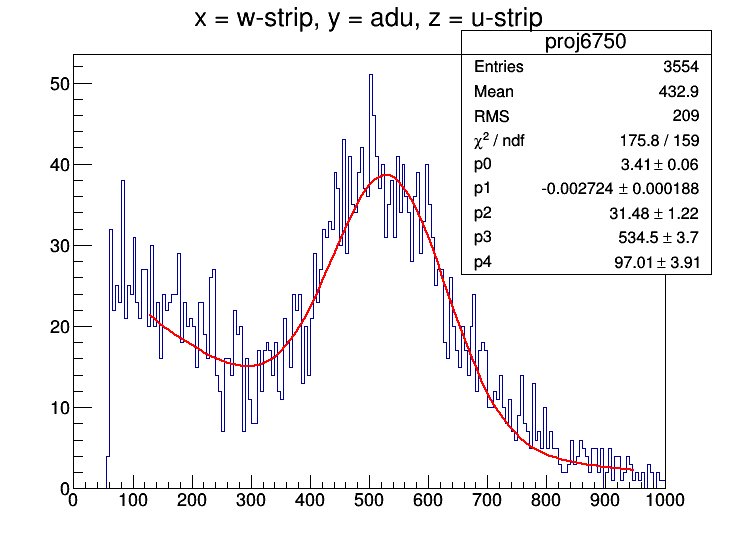
\includegraphics[width= 4in, keepaspectratio = true]{distribution}
    \caption{Example of ADC readout histogram from one U/W trapezoidal bin (U=67 W=50).  The red line is an exponential+gaussian fit.}
    \label{fig:distribution}
\end{figure}

\subsection{Fitting Strategy}

The Dalitz pixel cut works best when ADC threshold cuts can be placed close to the onset of the MIP peak in all three PMTs which view a given readout pixel.  This depends on all PMTs being well gain-matched and requires a knowledge of the light attenuation correction.  Since this is only approximately the case at the start of calibration, an iterative approach was used to progressively improve the MIP fit accuracy. 

For each iterative step, cuts to isolate the MIP peak energy are optimized using two cuts:
\begin{enumerate}
    \item Cuts on U,V,W MIP energy: A $3\sigma$ cut is placed on each MIP peak for PMTs contributing to the readout pixel based on gaussian fits.  The overall effect is to reduce the exponential background in the readout pixel. This improves the fits to some of the edges.
    \item Cuts on U+V+W MIP energy sum: The desired muon trajectory should deposit the same amount of energy into each U,V,W layer. After the initial $3\sigma$ cuts and fitting attenuation curves, individual gains can be estimated. Using the emperically found gains, a cut on the U,V,W sum of ADC signals is used to eliminate events whose partial U,V,W energies could not contribute to the sum.\end{enumerate}

\begin{figure}[h]
    \centering
    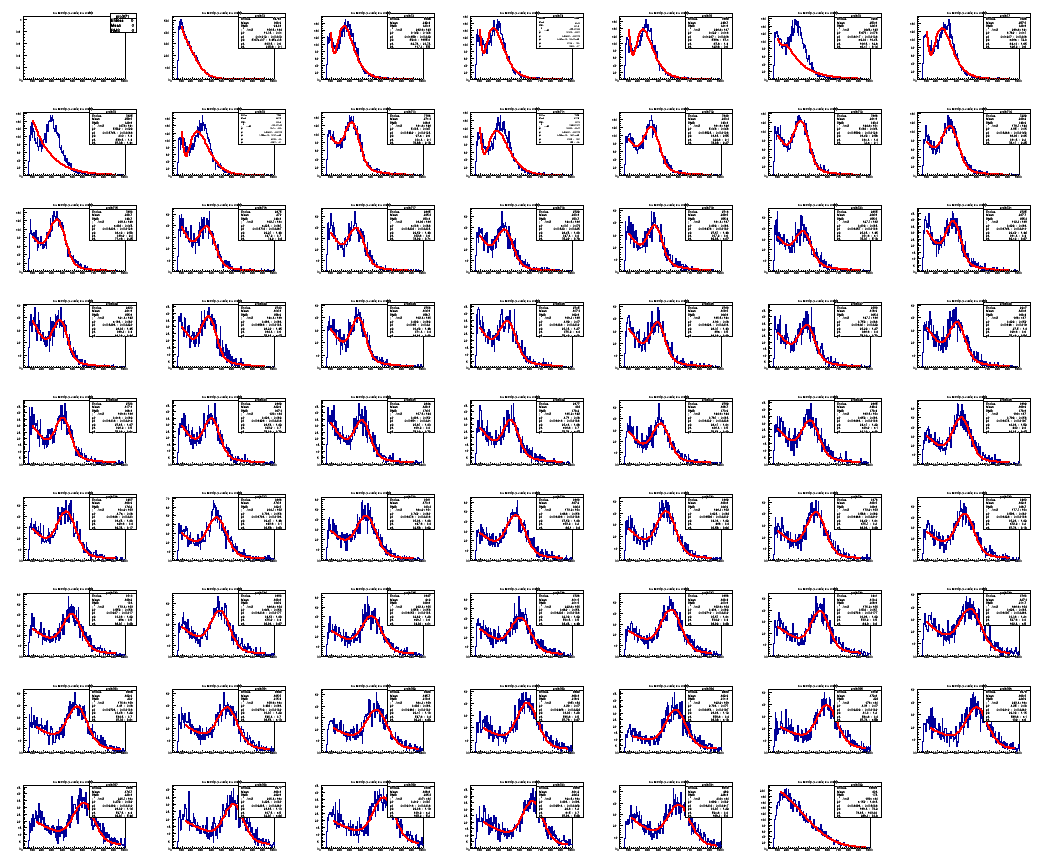
\includegraphics[width= 6in, keepaspectratio = true]{allstrip67}
    \caption{Example of all W crossing strip slices of the ADC readout from PMT U67.}
    \label{fig:allstrip67}
\end{figure}

\FloatBarrier
\subsection{Iteration Process}
For each iteration pass a $3\sigma$ cut on ADC distributions are made around the MIP peaks, determined by either the MIP signal fits or by attenuation fits.  This allows for a converging result because each cut on one U,V,W layer affects the other two. Therefore the MIP signal fits keeps improving as the attenuation fit and gains improve. 

To illustrate how the process works, the following section shows each pass of a typical iteration.  For each pass the cuts are described, followed by MIP fit plots for six representative U PMTs and a fixed crossing strip (W60).  Finally attenuation fits for each PMT are shown, which show how the multiple cuts affect each attenuation fit as a function of strip number. 

\clearpage
\FloatBarrier
\subsubsection{Pass 0}
\begin{itemize}
    \item Multiplicity Cut: Only events where one PMT fired for each strip were allowed.
    \item Dalitz Cut: An empircal distance sum was used to remove events that don't fall into 
    this range determined by Equation \ref{eq:totaldist}.
    \item Valid hit or near neighbor hit: Using generated events on a calculated skeleton of 
    the pcal, each pixel was determined to be valid or not. Extra uncertainty was allowed by 
    also marking nearest neighboring pixels.
\end{itemize}

\begin{figure}[h]
    \centering
    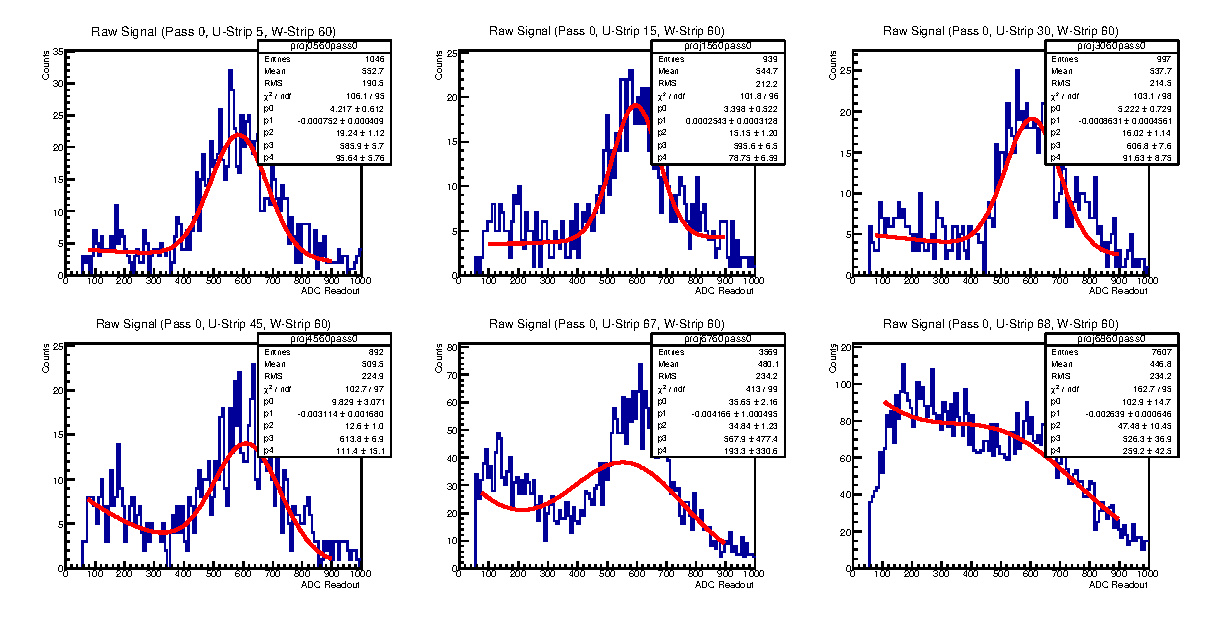
\includegraphics[height= 2.75in, keepaspectratio = true]{pass0}
    \caption{Shown is the ADC signal corresponding to signals from multiple u-strips 
    (5, 15, 30, 45, 67, and 68) and a projection of the w60 strip.}
    \label{fig:pass0}
\end{figure}

\begin{figure}[h]
    \centering
    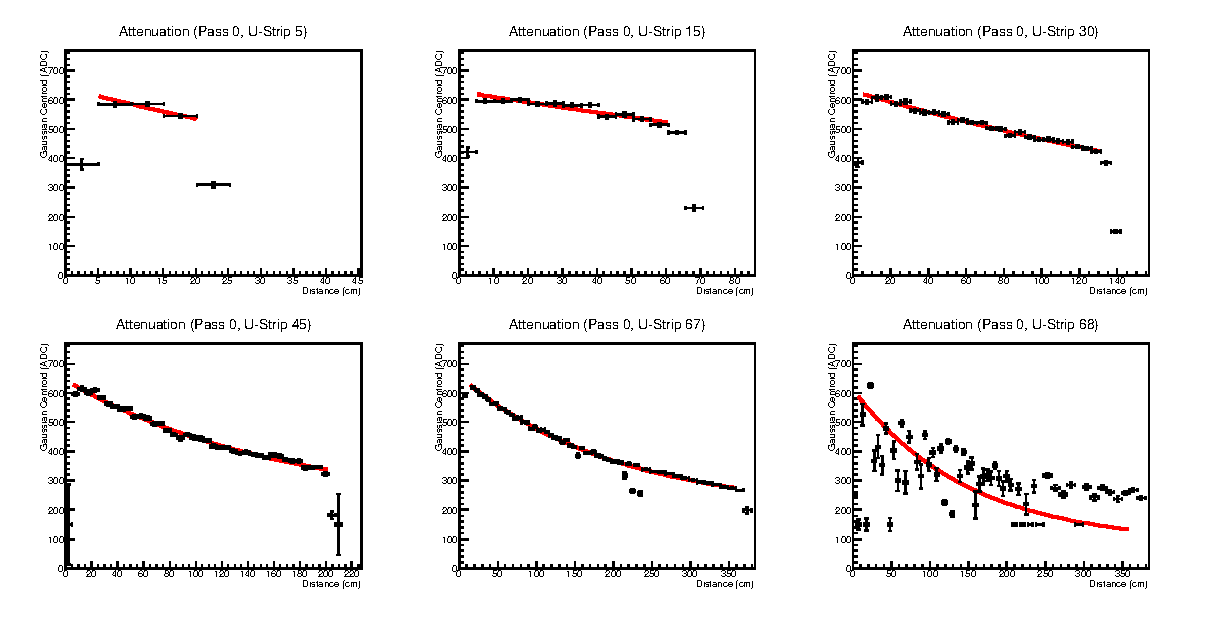
\includegraphics[height= 2.75in, keepaspectratio = true]{atpass0}
    \caption{Shown is the overall attenuation fits to the selected u-strips 
    (5, 15, 30, 45, 67, and 68).}
    \label{fig:atpass0}
\end{figure}


\clearpage
\FloatBarrier
\subsubsection{Pass 1}
\begin{itemize}
    \item Multiplicity Cut: Only events where one PMT fired for each strip were allowed.
    \item Dalitz Cut: An empircal distance sum was used to remove events that don't fall 
    into this range determined by Equation \ref{eq:totaldist}.
    \item Valid hit or near neighbor hit: Using generated events on a calculated skeleton
     of the pcal, each pixel was determined to be valid or not. Extra uncertainty was 
     allowed by also marking nearest neighboring pixels.
    \item 3$\sigma$ Cut on Signal: Each signal was fit to a Gaussian and exponential in 
    pass 0. The parameter $\sigma$ from the Gaussian fit was used to cut out the events
     that did not lie within this function.
\end{itemize}


\begin{figure}[h]
    \centering
    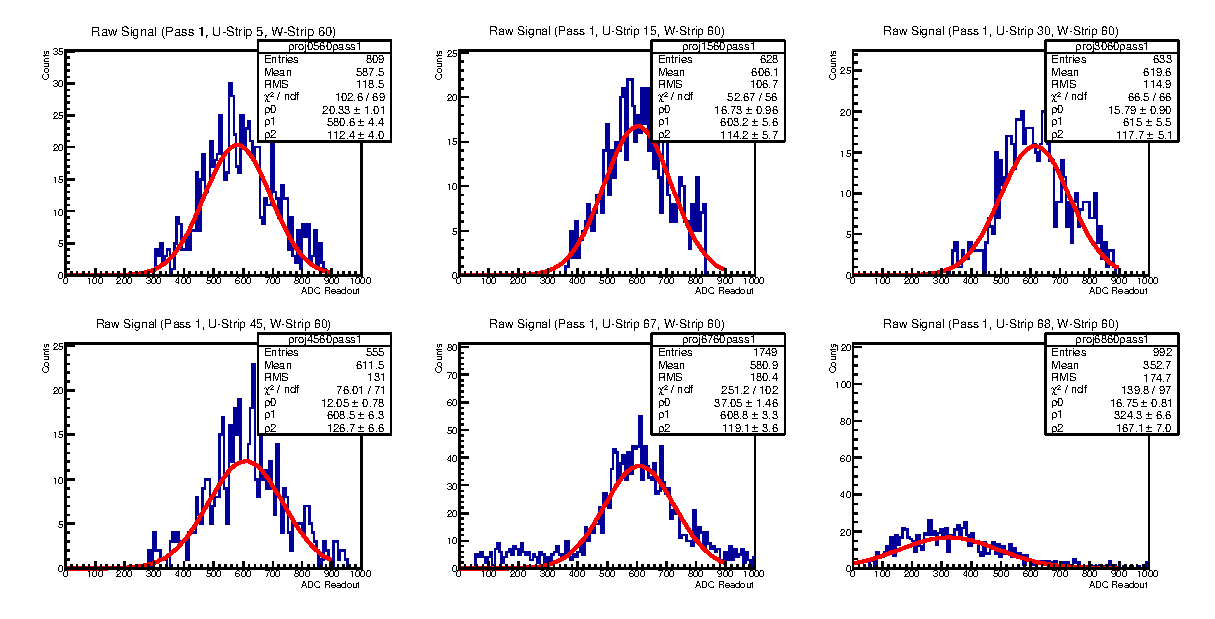
\includegraphics[height= 2.75in, keepaspectratio = true]{pass1}
    \caption{Shown is the ADC signal corresponding to signals from multiple u-strips
     (5, 15, 30, 45, 67, and 68) and a projection of the w60 strip.}
    \label{fig:pass1}
\end{figure}

\begin{figure}[h]
    \centering
    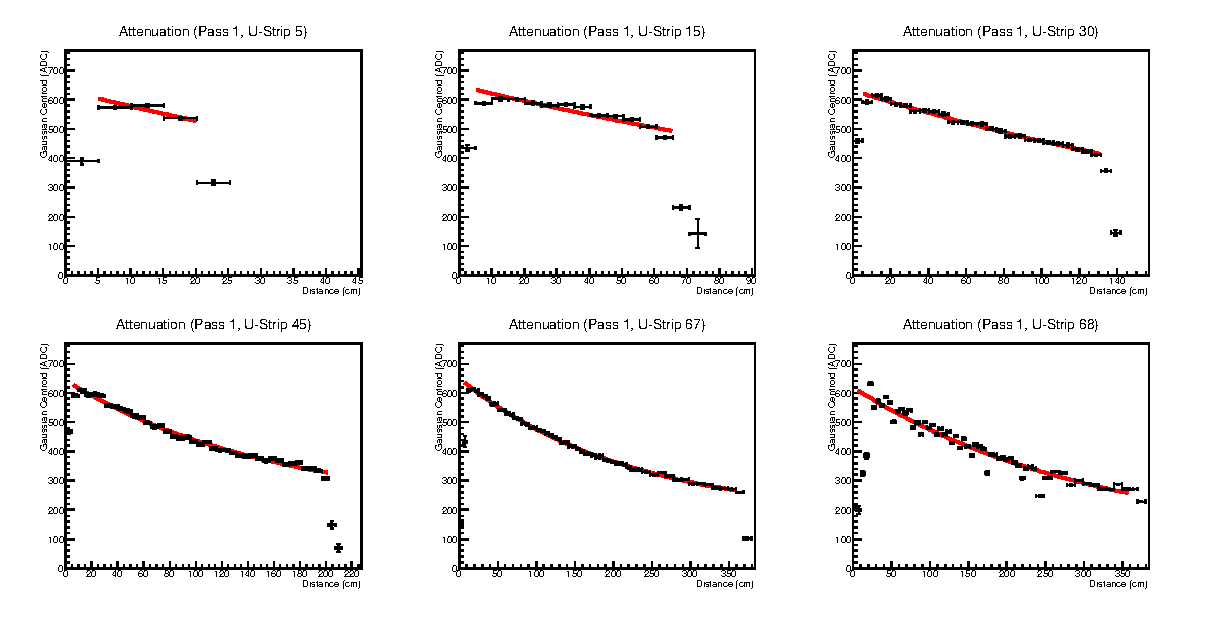
\includegraphics[height= 2.75in, keepaspectratio = true]{atpass1}
    \caption{Shown is the overall attenuation fits to the selected u-strips 
    (5, 15, 30, 45, 67, and 68).}
    \label{fig:atpass1}
\end{figure}



\clearpage
\FloatBarrier
\subsubsection{Pass 2}
\begin{itemize}
    \item Multiplicity Cut: Only events where one PMT fired for each strip were allowed.
    \item Dalitz Cut: An empircal distance sum was used to remove events that don't fall 
    into this range determined by Equation \ref{eq:totaldist}.
    \item Valid hit or near neighbor hit: Using generated events on a calculated skeleton 
    of the pcal, each pixel was determined to be valid or not. Extra uncertainty was allowed 
    by also marking nearest neighboring pixels.
    \item Cut on Attenuation Fits: When the signals where the Gaussian centroid from pass 1 
    were outside an ADC value of $\pm50$ from the attenuation fit, the obtained $\sigma$ was 
    ignored and a new cut about the attenuation fit was employed. If the centroid was close 
    to ADC value from the attenuation fit a 2$\sigma$ cut was used to remove extra background.
\end{itemize}


\begin{figure}[h]
    \centering
    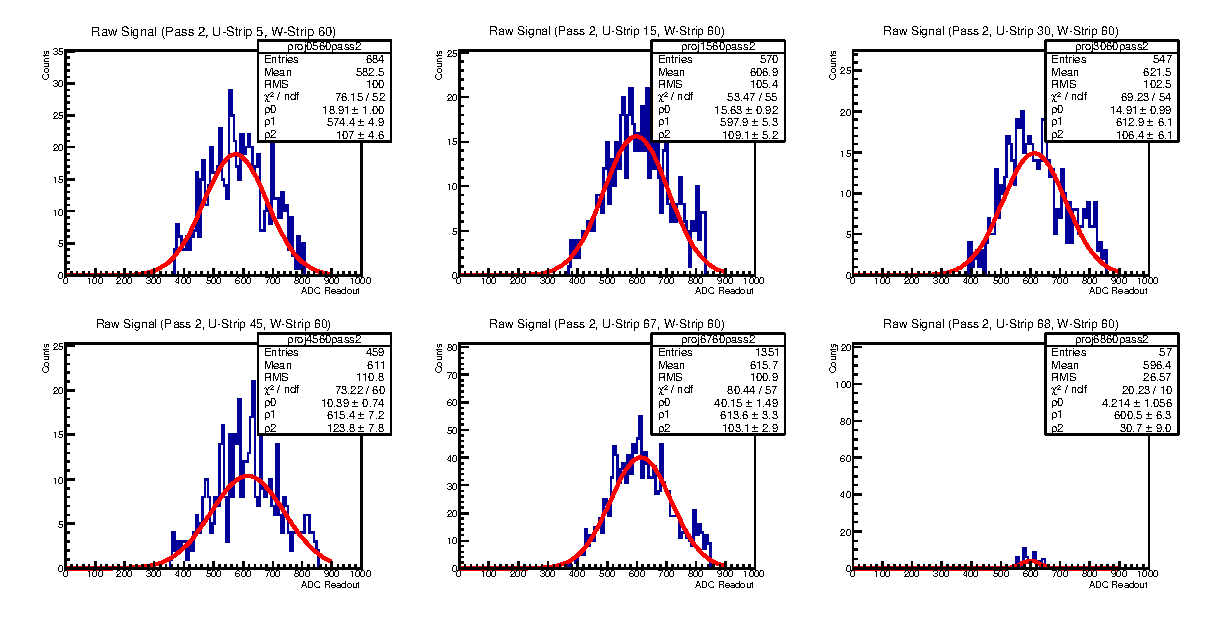
\includegraphics[height= 2.75in, keepaspectratio = true]{pass2}
    \caption{Shown is the ADC signal corresponding to signals from multiple u-strips 
    (5, 15, 30, 45, 67, and 68) and a projection of the w60 strip.}
    \label{fig:pass2}
\end{figure}

\begin{figure}[h]
    \centering
    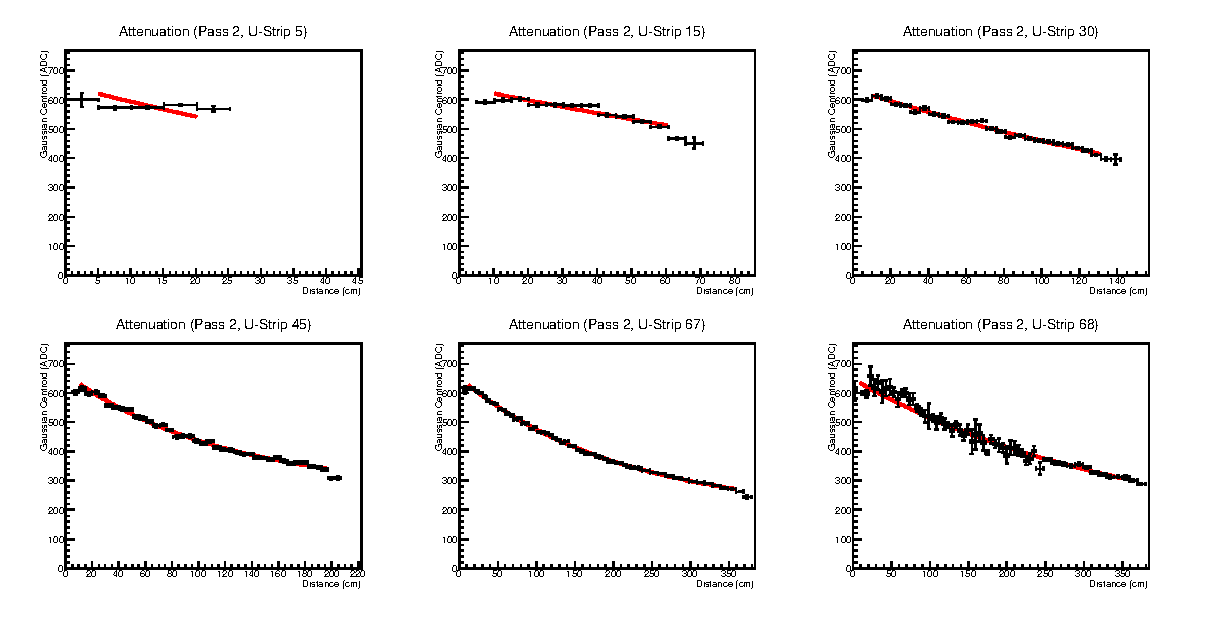
\includegraphics[height= 2.75in, keepaspectratio = true]{atpass2}
    \caption{Shown is the overall attenuation fits to the selected u-strips 
    (5, 15, 30, 45, 67, and 68).}
    \label{fig:atpass2}
\end{figure}



\clearpage
\FloatBarrier
\subsubsection{Pass 3}
\begin{itemize}
    \item Multiplicity Cut: Only events where one PMT fired for each strip were allowed.
    \item Dalitz Cut: An empircal distance sum was used to remove events that don't fall 
    into this range determined by Equation \ref{eq:totaldist}.
    \item Valid hit: Using generated events on a calculated skeleton of the pcal, each 
    pixel was determined to be valid or not.
    \item 3$\sigma$ Cut on Signal: Each signal was fit to a Gaussian in pass 2. The parameter 
    $\sigma$ from the Gaussian fit was used to cut out the events that did not lie within this function.
    \item Attenuation Corrected Intensity Cut: The ADC value measured was corrected with the 
    attenuation curves obtained from pass 2. The corrected value was summed over each layer. 
    A cut on this intensity was placed generously from 1300 to 2700
\end{itemize}

\begin{figure}[h]
    \centering
    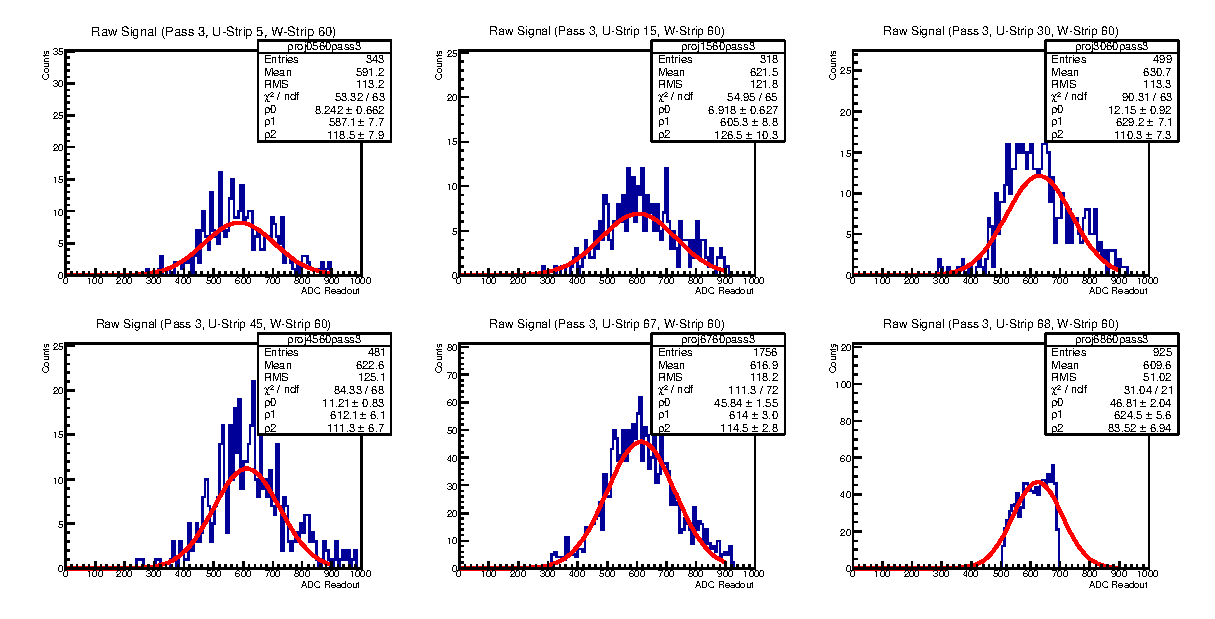
\includegraphics[height= 2.75in, keepaspectratio = true]{pass3}
    \caption{Shown is the ADC signal corresponding to signals from multiple u-strips 
    (5, 15, 30, 45, 67, and 68) and a projection of the w60 strip.}
    \label{fig:pass3}
\end{figure}

\begin{figure}[h]
    \centering
    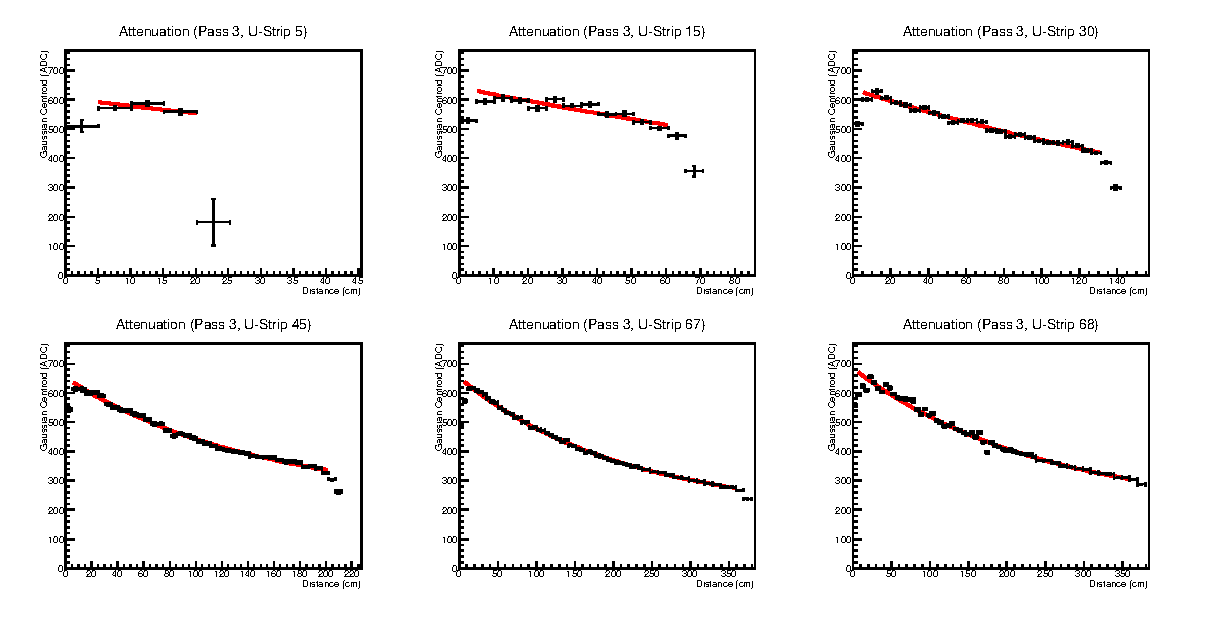
\includegraphics[height= 2.75in, keepaspectratio = true]{atpass3}
    \caption{Shown is the overall attenuation fits to the selected u-strips 
    (5, 15, 30, 45, 67, and 68).}
    \label{fig:atpass3}
\end{figure}

\clearpage
\FloatBarrier
\subsubsection{Pass 4}
\begin{itemize}
    \item Multiplicity Cut: Only events where one PMT fired for each strip were allowed.
    \item Dalitz Cut: An empircal distance sum was used to remove events that don't fall 
    into this range determined by Equation \ref{eq:totaldist}.
    \item Valid hit: Using generated events on a calculated skeleton of the pcal, each 
    pixel was determined to be valid or not.
    \item 3$\sigma$ Cut on Signal: Each signal was fit to a Gaussian in pass 2. The parameter 
    $\sigma$ from the Gaussian fit was used to cut out the events that did not lie within this function.
    \item Attenuation Corrected Intensity Cut: The ADC value measured was corrected with 
    the attenuation curves obtained from pass 2. The corrected value was summed over each 
    layer. A cut on this intensity was placed generously from 1300 to 2700
\end{itemize}


\begin{figure}[h]
    \centering
    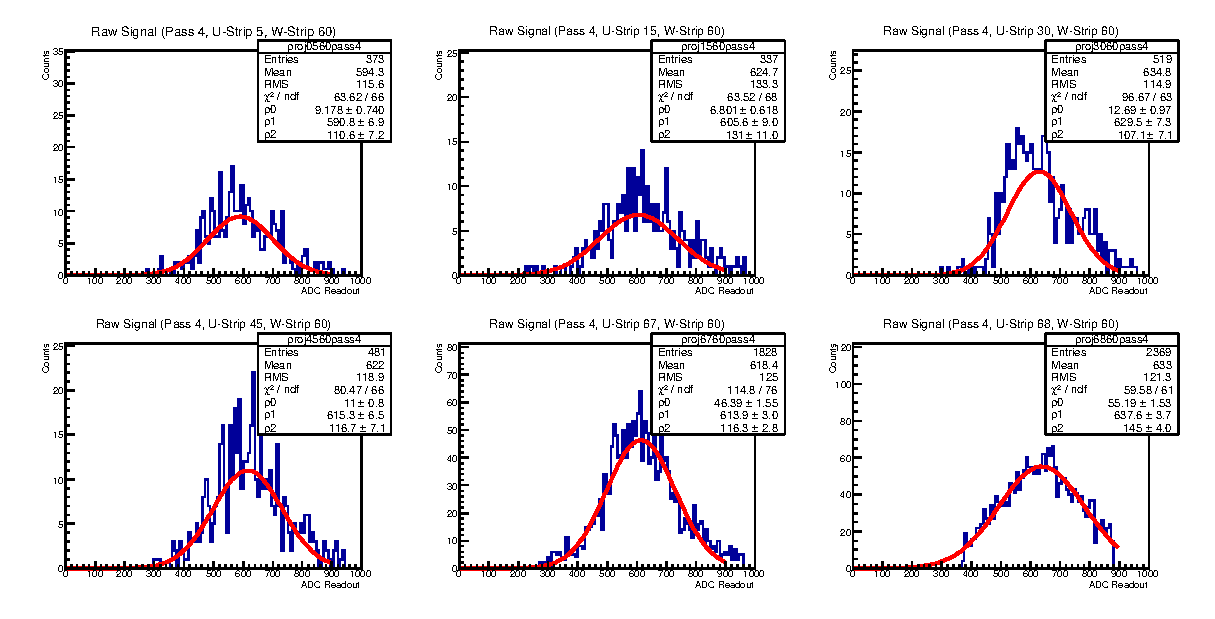
\includegraphics[height= 2.75in, keepaspectratio = true]{pass4}
    \caption{Shown is the ADC signal corresponding to signals from multiple u-strips (5, 15, 30, 45, 67, and 68) and a projection of the w60 strip.}
    \label{fig:pass4}
\end{figure}

\begin{figure}[h]
    \centering
    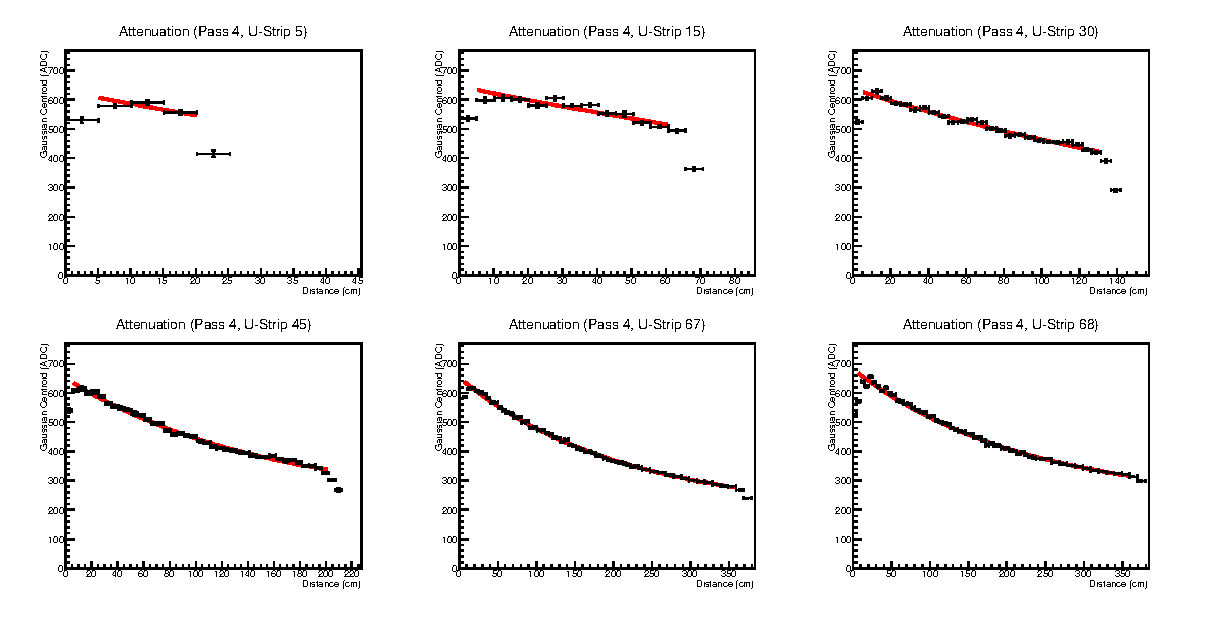
\includegraphics[height= 2.75in, keepaspectratio = true]{atpass4}
    \caption{Shown is the overall attenuation fits to the selected u-strips (5, 15, 30, 45, 67, and 68).}
    \label{fig:atpass4}
\end{figure}


\clearpage
\FloatBarrier
\subsubsection{Pass 5}
\begin{itemize}
    \item Multiplicity Cut: Only events where one PMT fired for each strip were allowed.
    \item Dalitz Cut: An empircal distance sum was used to remove events that don't fall 
    into this range determined by Equation \ref{eq:totaldist}.
    \item Valid hit: Using generated events on a calculated skeleton of the pcal, each pixel 
    was determined to be valid or not.
    \item 3$\sigma$ Cut on Signal: Each signal was fit to a Gaussian in pass 2. The parameter 
    $\sigma$ from the Gaussian fit was used to cut out the events that did not lie within this function.
    \item Attenuation Corrected Intensity Cut: The ADC value measured was corrected with the 
    attenuation curves obtained from pass 2. The corrected value was summed over each layer. 
    A cut on this intensity was placed generously from 1300 to 2700
\end{itemize}
               
               


\begin{figure}[h]
    \centering
    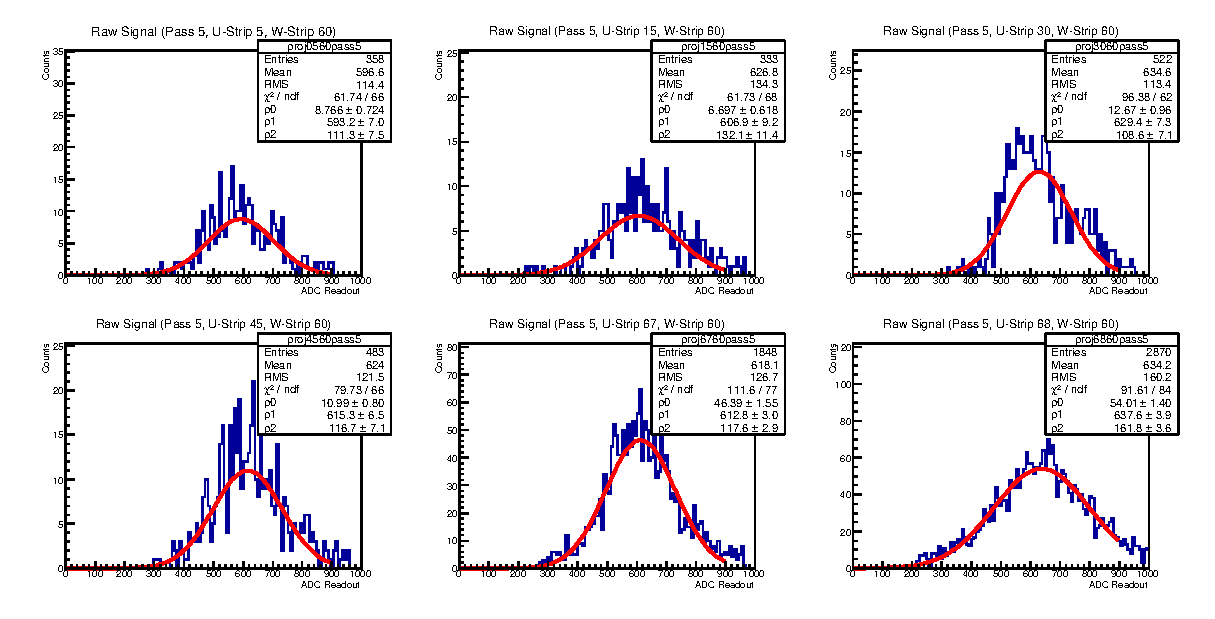
\includegraphics[height= 2.75in, keepaspectratio = true]{pass5}
    \caption{Shown is the ADC signal corresponding to signals from multiple u-strips 
    (5, 15, 30, 45, 67, and 68) and a projection of the w60 strip.}
    \label{fig:pass5}
\end{figure}

\begin{figure}[h]
    \centering
    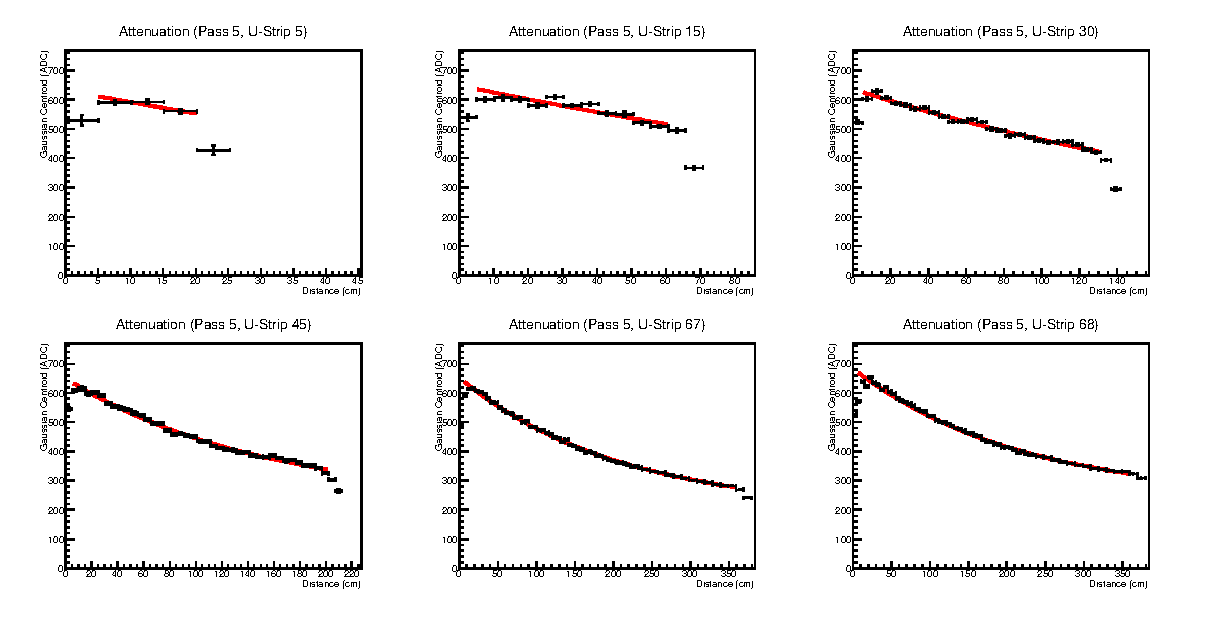
\includegraphics[height= 2.75in, keepaspectratio = true]{atpass5}
    \caption{Shown is the overall attenuation fits to the selected u-strips 
    (5, 15, 30, 45, 67, and 68).}
    \label{fig:atpass5}
\end{figure}


\FloatBarrier


\begin{figure}[h]
    \centering
    \begin{subfigure}[h]{0.3\textwidth}
        \centering
        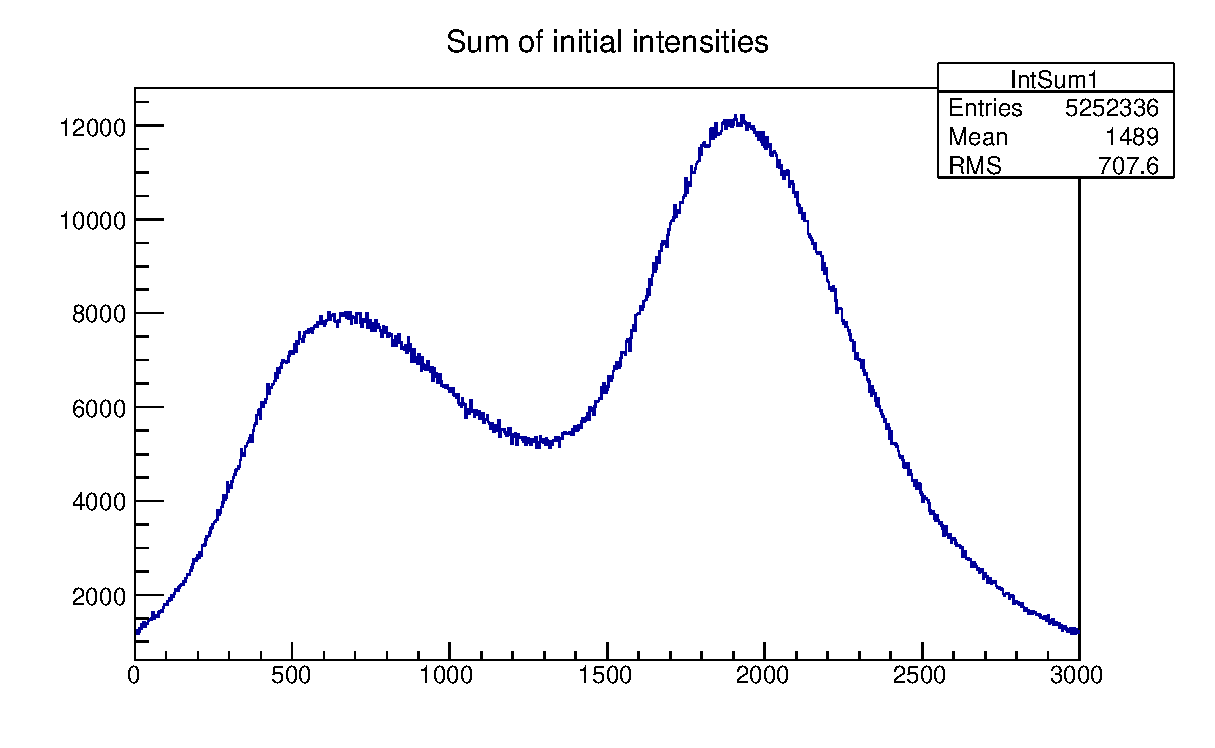
\includegraphics[width=\textwidth, keepaspectratio = true]{nocutsIsum}
        \caption{Sum of all initial intensities. No cuts.}
        \label{fig:nocutsIsum}
    \end{subfigure}
    ~
    \begin{subfigure}[h]{0.3\textwidth}
        \centering
        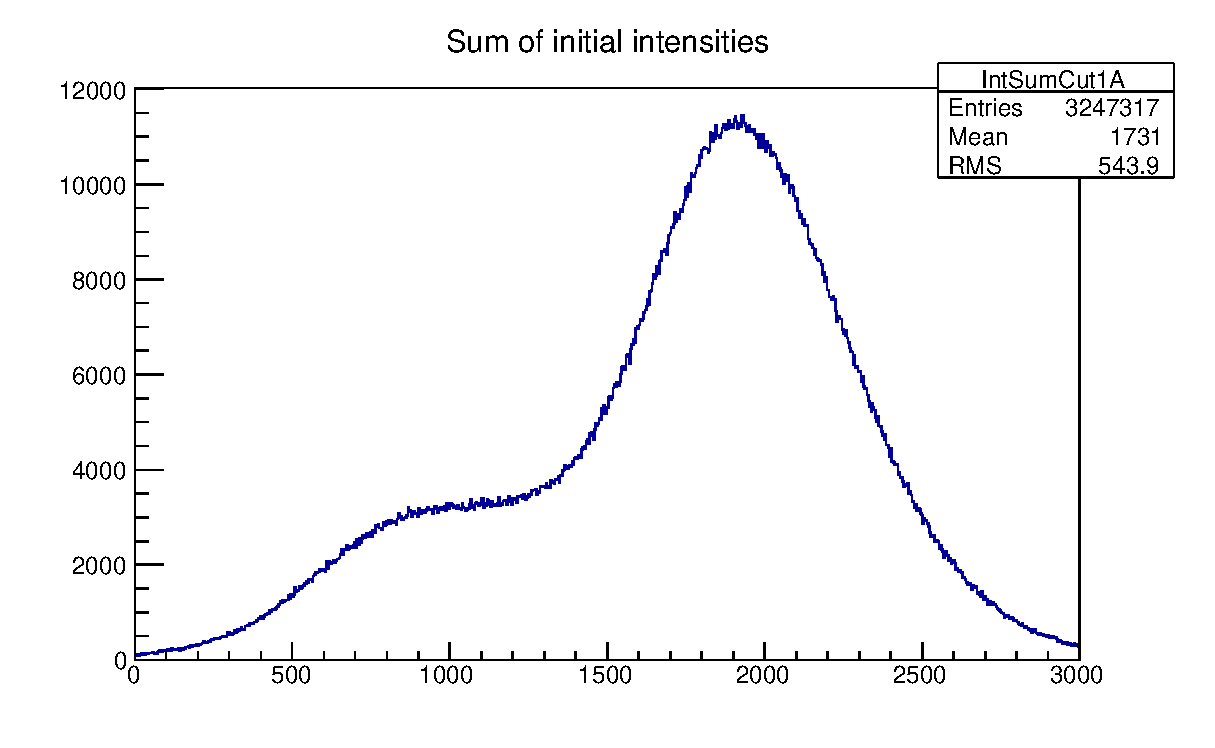
\includegraphics[width=\textwidth, keepaspectratio = true]{3sigcutIsum}
        \caption{Sum of all initial intensities. Three sigma Cut.}
        \label{fig:3sigcutIsum}
    \end{subfigure}
    ~
    \begin{subfigure}[h]{0.3\textwidth}
        \centering
        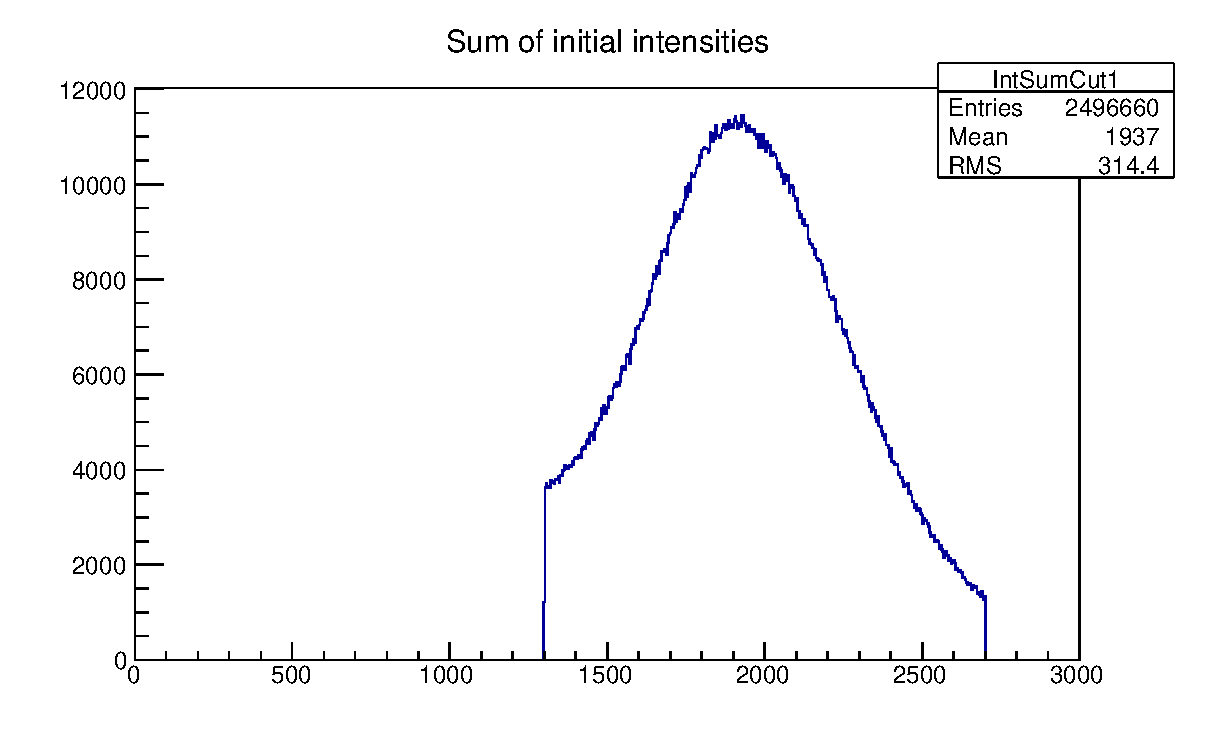
\includegraphics[width=\textwidth, keepaspectratio = true]{allcutsIsum}
        \caption{Sum of all initial intensities. Three sigma and sum Cut.}
        \label{fig:allcutsIsum}
    \end{subfigure}
    \caption{Sum of initial intensities should be near $650 \times 3 = 1950$ (after gain corrections).}
    \label{fig:intensities}
\end{figure}

\FloatBarrier
\subsection{Comparison of Fits}
Possibly the best evidence for needed cuts about each signal in an iterative process 
is seen by looking at the raw signal fits for a w strip with the possible u projections. 
These comparisons can be seen from pass 0 to pass 5 in Figures \ref{fig:w61sigfitpass0} and 
\ref{fig:w61sigfitpass5}. The difference between these signal tends to be cleaned up to a 
more Gaussian signal. By itself it is difficult to remove the backgound, but due to the correlating 
cuts on the u and v layers a reasonable output is produced.

\begin{figure}[h]
    \centering
    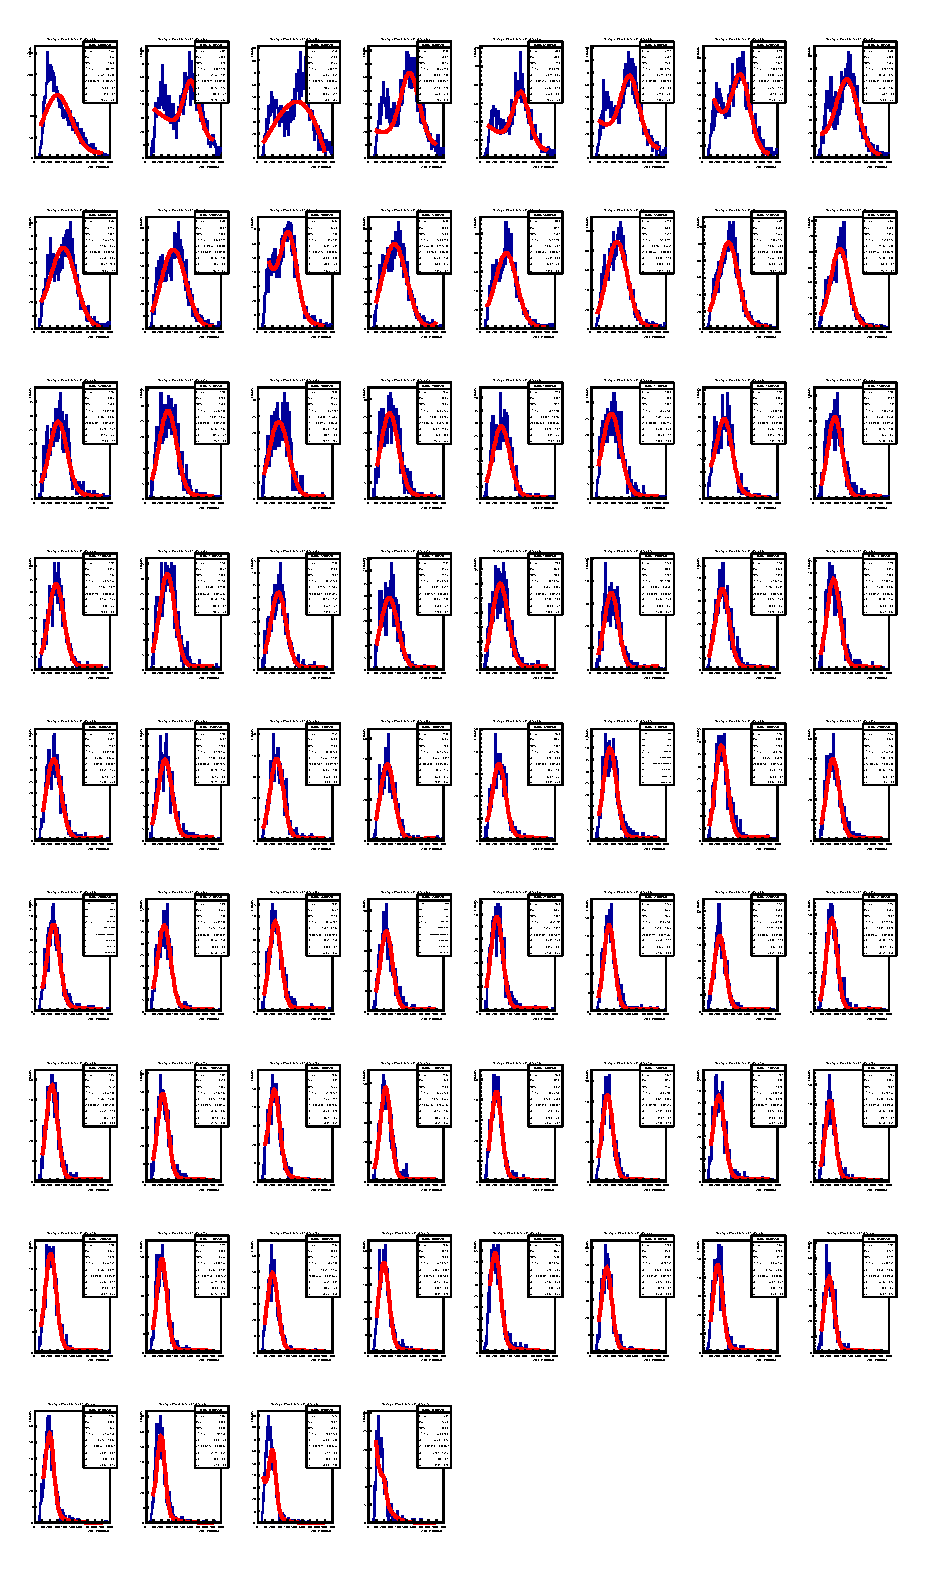
\includegraphics[width=\textwidth, height= 8in, keepaspectratio = true]{w61sigfitpass0}
    \caption{Shown is the ADC signal corresponding to signals from multiple u-strip projections of the w61 strip (pass0).}
    \label{fig:w61sigfitpass0}
\end{figure}

\begin{figure}[h]
    \centering
    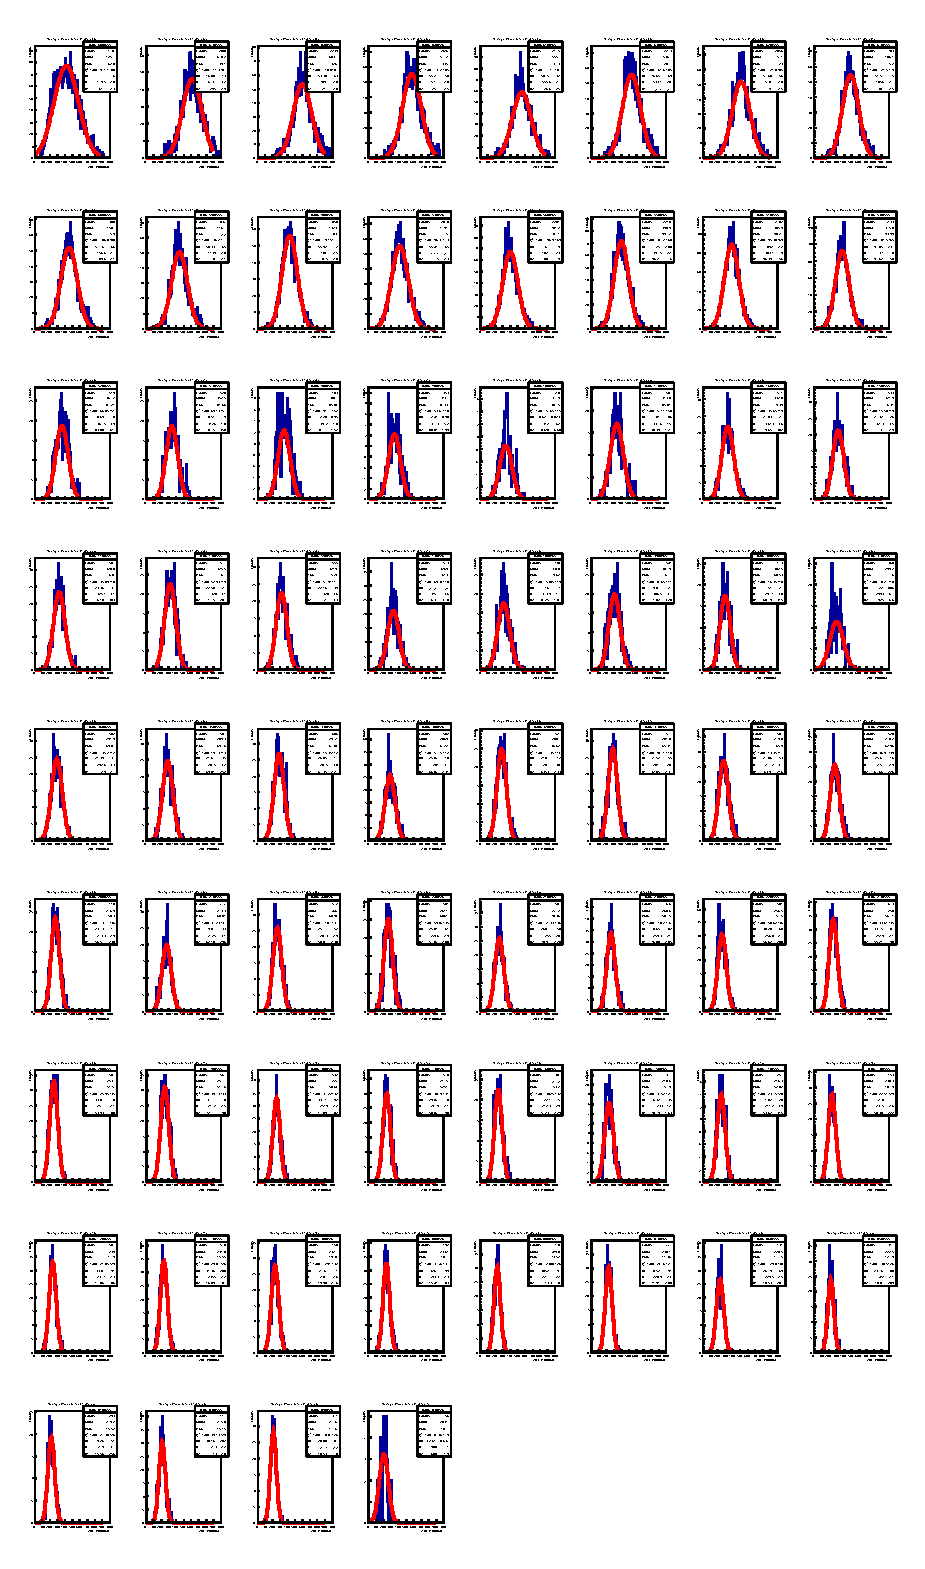
\includegraphics[width=\textwidth, height= 8in, keepaspectratio = true]{w61sigfitpass5}
    \caption{Shown is the ADC signal corresponding to signals from multiple u-strip projections of the w61 strip (pass5).}
    \label{fig:w61sigfitpass5}
\end{figure}


\FloatBarrier









\FloatBarrier
\subsection{Fit Function}
\FloatBarrier
The fit function suggested in the geometry note is an  exponential (equation \ref{eq:exp}).
It is also suggested that here the distance, $L$, should include the distance from the end of the strip 
to the cosmic ray track, $L_{s}$, as well as the extra fiber length, $L_{f}$.
In other words $L = L_{s} + L_{f}$.
However to analyze the quality of fit $L_{f}$ can be treated as a constant and absorbed into the parameter 
$a$ in equation \ref{eq:exp}.

\begin{equation}
    I = e^{a + bL}
    \label{eq:exp}
\end{equation}

\begin{figure}[h]
    \centering
 %   \begin{subfigure}[h]{0.4\textwidth}
        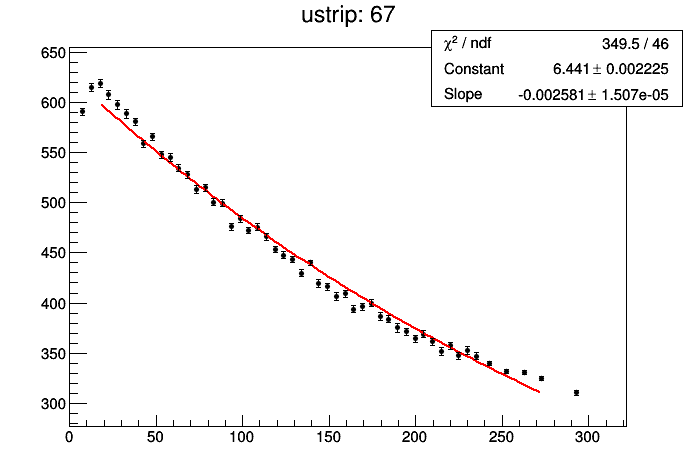
\includegraphics[width= \textwidth, keepaspectratio = true]{exponetial67}
        \caption{Shown is a fit with equation \ref{eq:exp}, where the y axis is the ADC value and the x axis is $L_{s}$.}
        \label{fig:exponential67}
%    \end{subfigure}
    ~
%    \begin{subfigure}[h]{0.4\textwidth}
%        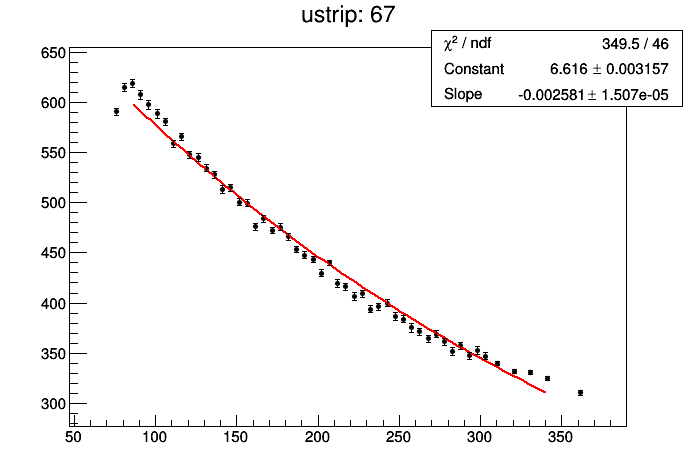
\includegraphics[width= \textwidth, keepaspectratio = true]{exponetialwfib67}
%        \caption{Shown is a fit with equation \ref{eq:exp}, where the y axis is the ADC value and the x axis is $L_{s} + L_{f}$.}
%        \label{fig:exponentialwfib67}
%    \end{subfigure}
%    \caption{Plotted is the fit of equation \ref{eq:exp}, where $L = L_{s}$ (a) and $L = L_{s} + L_{f}$ (b).}
%    \label{fig:expfit}
\end{figure}

As seen by figure \ref{fig:expfit}, a single exponential may not be the best fit for the data.
One might suggest a fitting function similar to equation \ref{eq:try1}, in order to separate the fiber 
attenuation from the scintillator attenuation.
However this function again can reduce to equation \ref{eq:exp} because $L_{f}$ is a constant for each 
scintillator strip and is seen not to be a good fit.


%\begin{equation}
%    \begin{split}
%        I &= a_{1}e^{b_{1}(L_{s} + L_{f})}e^{b_{2}L_{s}} \\
%          &= a_{1}e^{b_{1}(L_{s} + L_{f}) + b_{2}L_{s}} \\
%          &= a_{1}e^{(b_{1} + b_{2})L_{s} + b_{1}L_{f}} \\
%          &= a_{1}e^{b_{1}L_{f}}e^{(b_{1} + b_{2})L_{s}} \\
%          &= e^{a}e^{(b_{1} + b_{2})L_{s}} \\
%          &= e^{a}e^{bL_{s}} \\
%          &= e^{a + bL_{s}} \\
%    \end{split}
%    \label{eq:try1}
%\end{equation}

\begin{comment}
\begin{equation}
    I(L_{s})= ae^{(b_{1} + b_{2})L_{s} + b_{1}L_{f}}
    \label{eq:try1mid}
\end{equation}

\FloatBarrier
\begin{figure}[h]
    \centering
    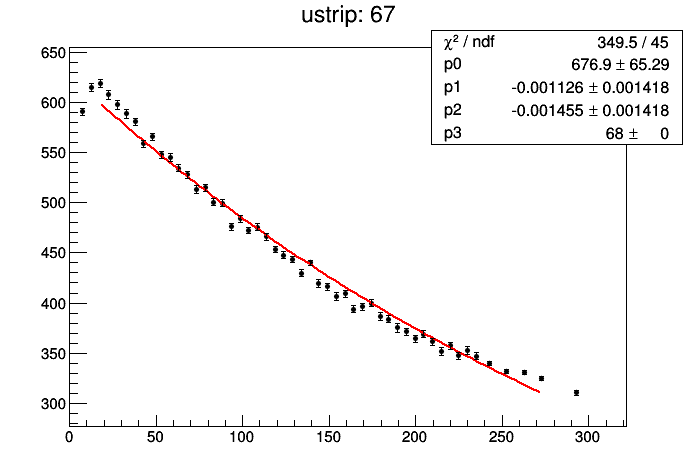
\includegraphics[width= 3in, keepaspectratio = true]{exponential67eq9}
    \caption{Plotted is the fit of equation \ref{eq:try1mid} as a function of $L_{s}$.}
    \label{fig:try1mid}
\end{figure}
\end{comment}
\FloatBarrier


Other functional forms that could represent the data should be similar to that of an exponential.
A couple of these forms include an exponential plus a constant or a sum of exponentials.
In both cases, some considerations have to be made on the domain of the function.
The sum of two exponentials was considered to have some portion of the attenuation in the fibers to 
be different than inside the scintillator. This does not get a better fit, and does not allow any more 
information to be extracted. Therefore the function used in fitting the attenuation was chosen to be 
an exponential with an added constant as seen by Equation \ref{eq:expplusconst}.

\begin{equation}
    I(L_{s}) = ae^{bL_{s}}+c
    \label{eq:expplusconst}
\end{equation}


\FloatBarrier
\subsection{Calibration Constants}
A table of constants can be uploaded to the clas12 database once the fitting procedure is complete.
%To get the calibration constants below, parameter limits were set on equation \ref{eq:expplusconst} 
%for $200.0 < a < 900.0$, $-0.009 < b < -0.0005$, and $0.0 < c < 700.0$, based on qualitative observation on a global fit.
For strips where fewer than five points were available for fitting, either 
a single exponential or a constant term was used for the fitting function. This was done to avoid overconstraining the fit. All the fits shown are for Sector One of the PCAL.
\FloatBarrier
\vspace{5mm}

%Ufits:
\begin{figure}[h]
    \centering
    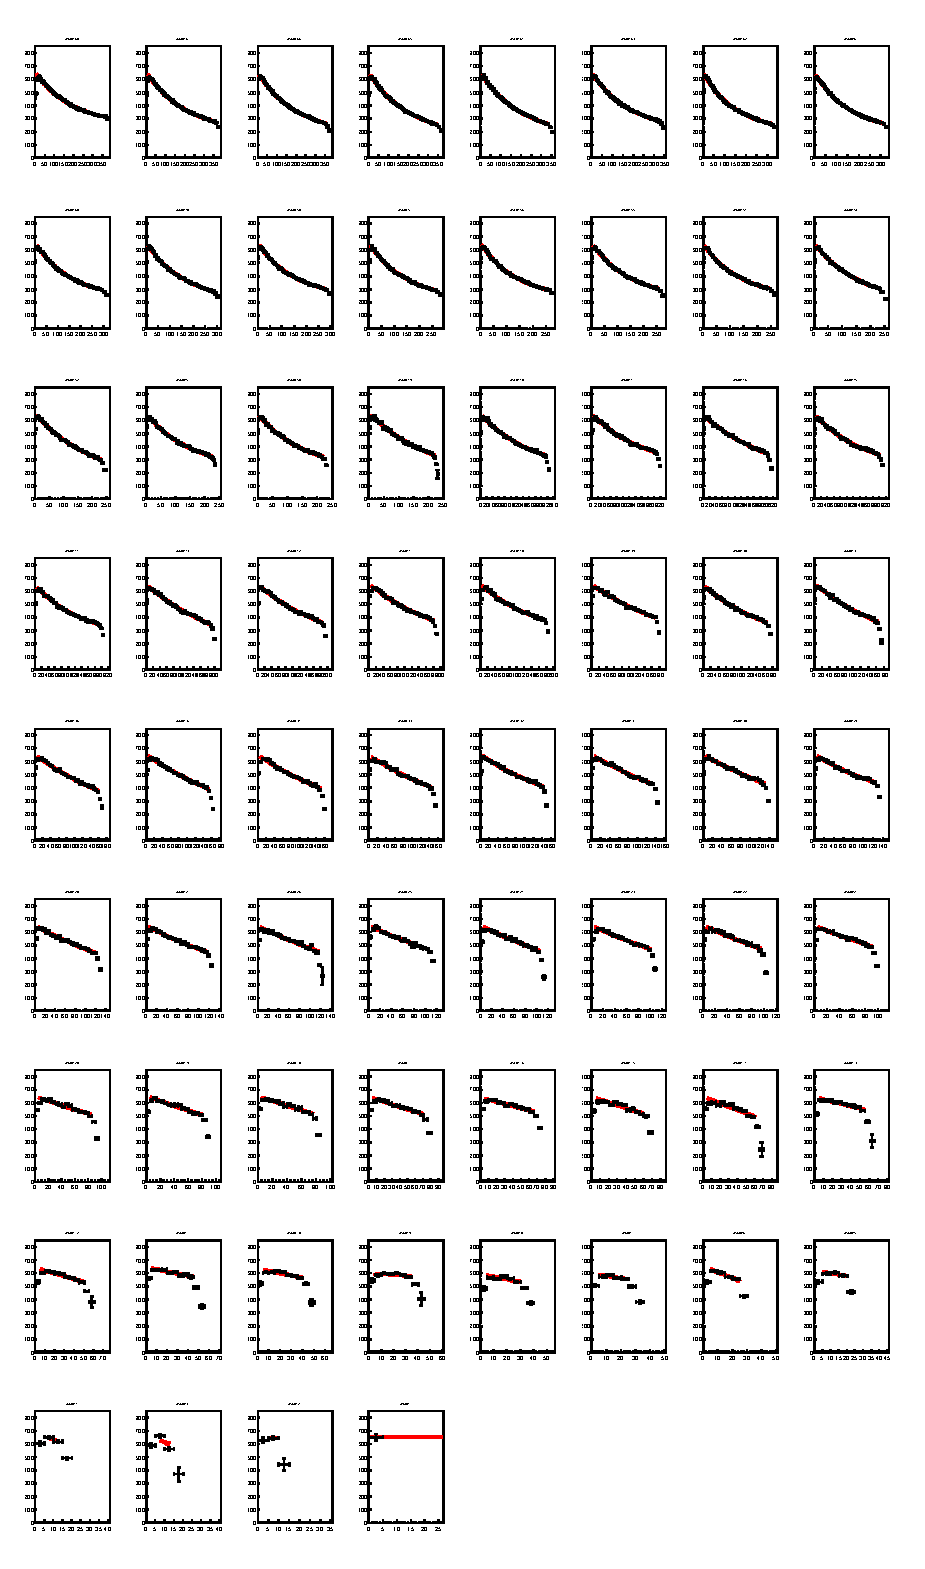
\includegraphics[width= 6.5in, height = 8in, keepaspectratio = true]{allustrips}
    \caption{Attenuation fits for U strips with U68 in the upper left hand corner. Y-axis is linear ranging from 0 to 850. X-axis varies 
    depending on the number of points in the plot.}
    \label{fig:allustrips}
\end{figure}

\FloatBarrier
%Vfits:
\begin{figure}[h]
    \centering
    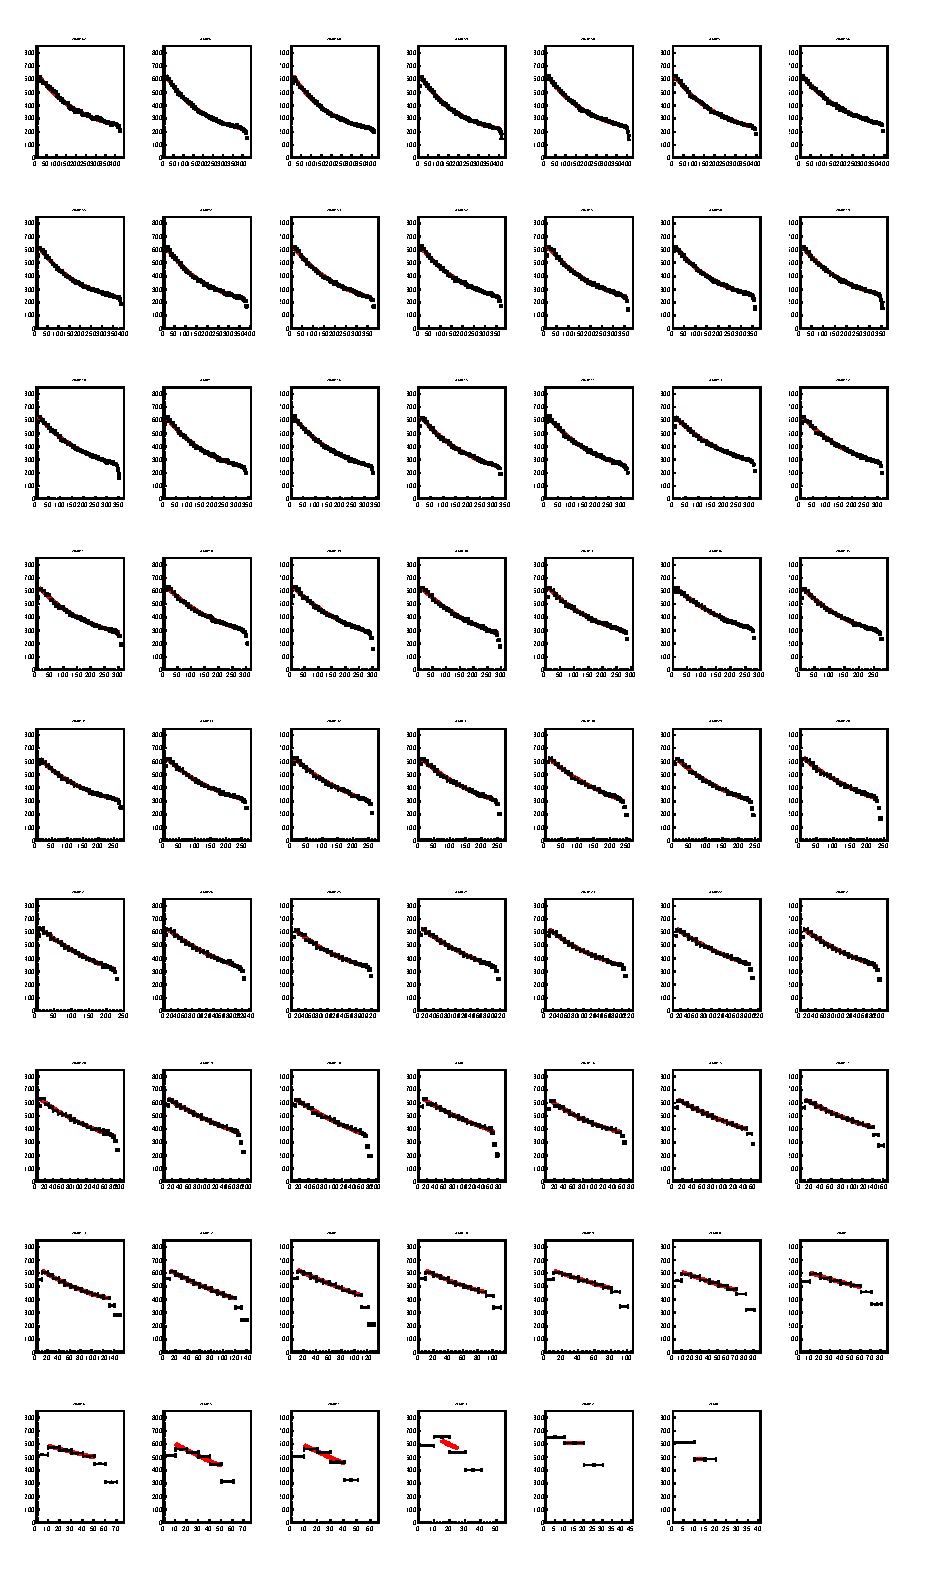
\includegraphics[width= 6.5in, height = 8in, keepaspectratio = true]{allvstrips}
    \caption{Attenuation fits for V strips V62 in the upper left hand corner. Y-axis is linear ranging from 0 to 850. X-axis varies 
    depending on the number of points in the plot.}
    \label{fig:allvstrips}
\end{figure}


\FloatBarrier

%Wfits:
\begin{figure}[h]
    \centering
    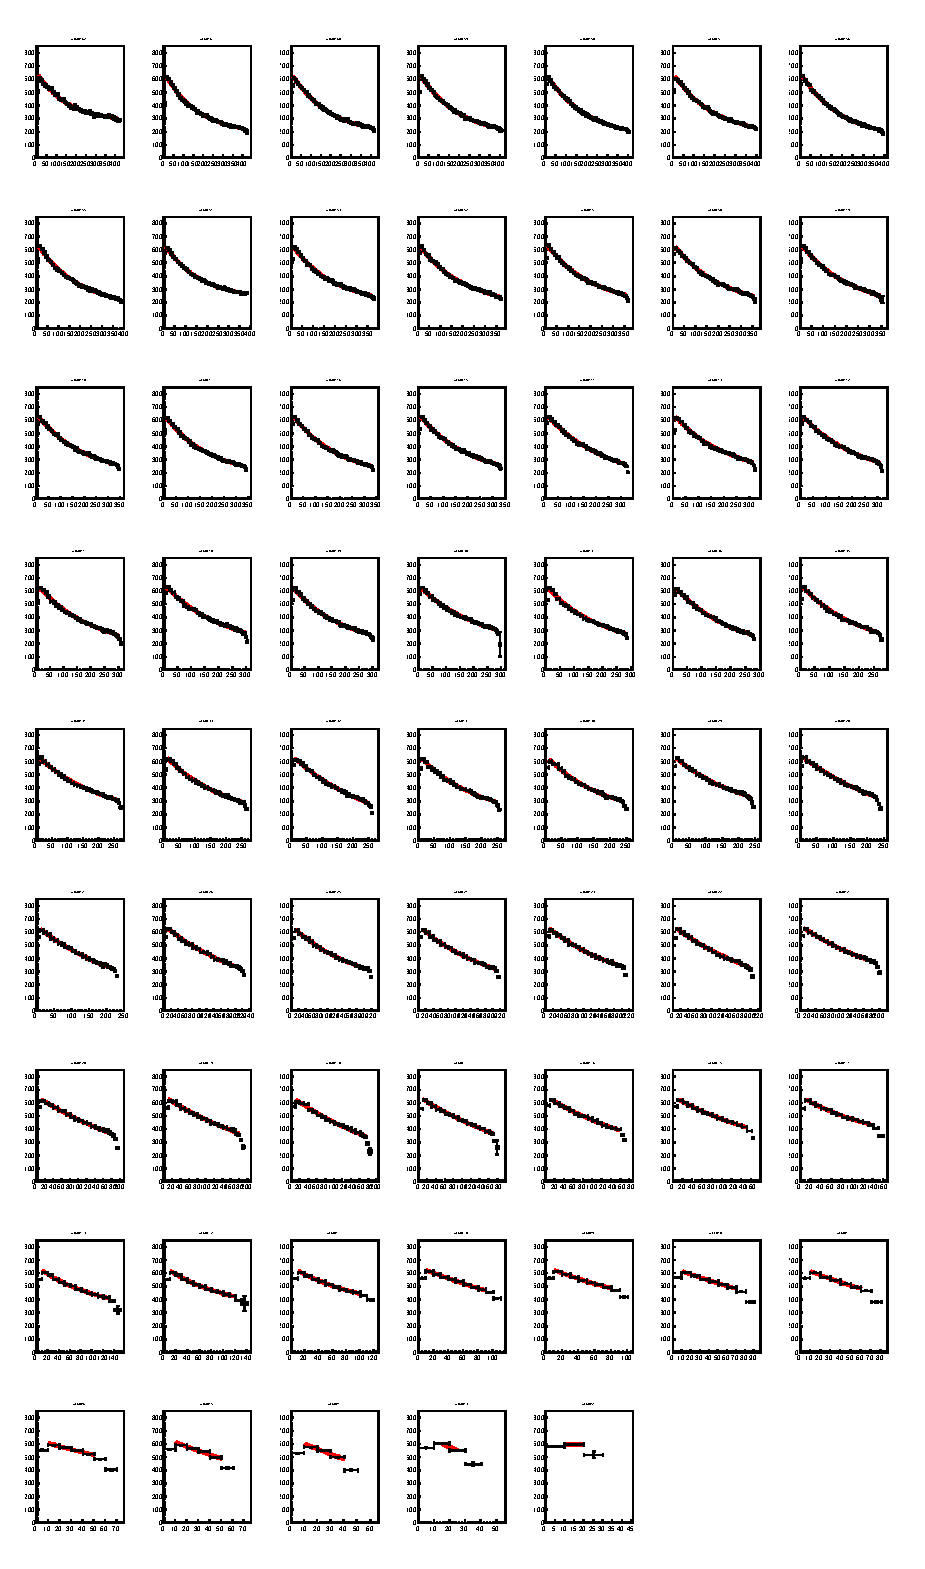
\includegraphics[width= 6.5in, height = 8in, keepaspectratio = true]{allwstrips}
    \caption{Attenuation fits for V strips V62 in the upper left hand corner. Y-axis is linear ranging from 0 to 850. X-axis varies 
    depending on the number of points in the plot.}
    \label{fig:allustrips}
\end{figure}

\FloatBarrier
\begin{table}[h]
        \centering{}
        \scalebox{0.75}{
        \begin{tabular}{|c|c|c|c|}
            \hline
            U-Strip &  Parameter $a$  &Parameter $b$  & Parameter $c$ \\ \hline
1   &   650   &   0   &   0  \\  \hline  
2   &   650   &   0   &   0  \\  \hline  
3   &   650   &   -0.009   &   0  \\  \hline  
4   &   650   &   -0.009   &   0  \\  \hline  
5   &   616.113   &   -0.00639717   &   33.8858  \\  \hline  
6   &   649.996   &   -0.00717551   &   0.0046356  \\  \hline  
7   &   649.968   &   -0.00318808   &   0.0319326  \\  \hline  
8   &   649.972   &   -0.00232476   &   0.0273016  \\  \hline  
9   &   649.146   &   -0.00112904   &   0.854413  \\  \hline  
10   &   649.999   &   -0.00281005   &   0.000286188  \\  \hline  
11   &   649.993   &   -0.00286292   &   0.00718601  \\  \hline  
12   &   650   &   -0.0041656   &   0.000445736  \\  \hline  
13   &   650   &   -0.003283   &   0.000103724  \\  \hline  
14   &   649.997   &   -0.00376077   &   5.37227e-06  \\  \hline  
15   &   650.001   &   -0.00339912   &   6.96689e-06  \\  \hline  
16   &   649.997   &   -0.00305411   &   8.14649e-06  \\  \hline  
17   &   649.999   &   -0.00345134   &   9.95183e-09  \\  \hline  
18   &   649.998   &   -0.00310718   &   4.19396e-07  \\  \hline  
19   &   650   &   -0.00311517   &   5.01049e-06  \\  \hline  
20   &   650   &   -0.00281725   &   6.09084e-06  \\  \hline  
21   &   650   &   -0.00315783   &   3.38135e-05  \\  \hline  
22   &   650   &   -0.00328681   &   2.55834e-08  \\  \hline  
23   &   650   &   -0.00316776   &   2.15877e-05  \\  \hline  
24   &   649.999   &   -0.00317021   &   4.66803e-05  \\  \hline  
25   &   650   &   -0.00327065   &   5.9556e-06  \\  \hline  
26   &   650.001   &   -0.00309179   &   1.40689e-08  \\  \hline  
27   &   551.087   &   -0.00385902   &   98.9141  \\  \hline  
28   &   649.997   &   -0.00307714   &   7.49416e-05  \\  \hline  
29   &   419.522   &   -0.00552754   &   230.477  \\  \hline  
30   &   650   &   -0.00316014   &   0.000130702  \\  \hline  
31   &   650.001   &   -0.00312815   &   2.25921e-06  \\  \hline  
32   &   585.658   &   -0.00373922   &   64.3455  \\  \hline  
33   &   581.001   &   -0.00374214   &   68.997  \\  \hline  
34   &   650.002   &   -0.00328878   &   0.000131253  \\  \hline  
35   &   650   &   -0.00332314   &   1.43305e-05  \\  \hline  
36   &   649.998   &   -0.00340294   &   1.07435e-07  \\  \hline  
37   &   556.399   &   -0.00428136   &   93.5991  \\  \hline  
38   &   483.854   &   -0.00534903   &   166.146  \\  \hline  
39   &   482.458   &   -0.00431684   &   167.541  \\  \hline  
40   &   392.765   &   -0.00669036   &   257.235  \\  \hline  
41   &   499.22   &   -0.00443664   &   150.78  \\  \hline  
42   &   513.839   &   -0.00445738   &   136.164  \\  \hline  
43   &   581.507   &   -0.00388427   &   68.4914  \\  \hline  
44   &   391.463   &   -0.00757633   &   258.536  \\  \hline  
45   &   434.393   &   -0.00632194   &   215.608  \\  \hline  
46   &   463.813   &   -0.00513914   &   186.187  \\  \hline  
47   &   413.809   &   -0.00605594   &   236.189  \\  \hline  
48   &   442.234   &   -0.00592955   &   207.766  \\  \hline  
49   &   509.976   &   -0.00449146   &   140.024  \\  \hline  
50   &   443.895   &   -0.00614484   &   206.105  \\  \hline  
51   &   425.765   &   -0.00641114   &   224.233  \\  \hline  
52   &   504.812   &   -0.00511618   &   145.188  \\  \hline  
53   &   454.838   &   -0.0061679   &   195.162  \\  \hline  
54   &   406.411   &   -0.00766326   &   243.589  \\  \hline  
55   &   415.976   &   -0.00690821   &   234.026  \\  \hline  
56   &   421.326   &   -0.00710769   &   228.675  \\  \hline  
57   &   435.635   &   -0.00660386   &   214.362  \\  \hline  
58   &   411.518   &   -0.00663318   &   238.483  \\  \hline  
59   &   438.882   &   -0.00625669   &   211.118  \\  \hline  
60   &   423.763   &   -0.00618908   &   226.238  \\  \hline  
61   &   444.671   &   -0.0063621   &   205.328  \\  \hline  
62   &   438.481   &   -0.00674885   &   211.519  \\  \hline  
63   &   437.138   &   -0.00564978   &   212.862  \\  \hline  
64   &   482.525   &   -0.00495599   &   167.473  \\  \hline  
65   &   473.388   &   -0.00516614   &   176.613  \\  \hline  
66   &   465.633   &   -0.00500512   &   184.367  \\  \hline  
67   &   455.941   &   -0.00479029   &   194.059  \\  \hline  
68   &   410.201   &   -0.00506009   &   239.798  \\  \hline  
        \end{tabular}
        }
        \caption{Calibration Constants for the U layer.}
        \label{tab:UattenC}
\end{table}


\begin{table}[h]
        \centering
        \scalebox{0.75}{
        \begin{tabular}{|c|c|c|c|}
            \hline
            V-Strip &  Parameter $a$  &Parameter $b$  & Parameter $c$ \\ \hline
1   &   650.002   &   0   &   0  \\  \hline  
2   &   649.999   &   0   &   0  \\  \hline  
3   &   650.001   &   -0.009   &   0  \\  \hline  
4   &   650.001   &   -0.009   &   8.41036e-07  \\  \hline  
5   &   650   &   -0.00794645   &   5.04738e-06  \\  \hline  
6   &   649.225   &   -0.00402729   &   0.773706  \\  \hline  
7   &   341.165   &   -0.009   &   308.835  \\  \hline  
8   &   649.999   &   -0.0043402   &   0.000921065  \\  \hline  
9   &   650   &   -0.00346629   &   0.00030414  \\  \hline  
10   &   409.661   &   -0.0073313   &   240.338  \\  \hline  
11   &   650   &   -0.0036951   &   0.000157707  \\  \hline  
12   &   543.255   &   -0.00487653   &   106.745  \\  \hline  
13   &   385.429   &   -0.00755387   &   264.571  \\  \hline  
14   &   462.536   &   -0.00523798   &   187.463  \\  \hline  
15   &   490.318   &   -0.00478212   &   159.682  \\  \hline  
16   &   409.407   &   -0.00682511   &   240.592  \\  \hline  
17   &   644.496   &   -0.00311038   &   5.50402  \\  \hline  
18   &   649.997   &   -0.00345834   &   1.60129e-06  \\  \hline  
19   &   650   &   -0.00314254   &   4.40293e-06  \\  \hline  
20   &   476.84   &   -0.00525174   &   173.161  \\  \hline  
21   &   504.696   &   -0.00482932   &   145.304  \\  \hline  
22   &   501.641   &   -0.00447931   &   148.359  \\  \hline  
23   &   427.011   &   -0.00618067   &   222.989  \\  \hline  
24   &   532.597   &   -0.00429752   &   117.404  \\  \hline  
25   &   452.731   &   -0.00555935   &   197.267  \\  \hline  
26   &   514.63   &   -0.00444436   &   135.371  \\  \hline  
27   &   562.158   &   -0.00411837   &   87.8438  \\  \hline  
28   &   552.525   &   -0.00397784   &   97.4754  \\  \hline  
29   &   505.009   &   -0.00490977   &   144.992  \\  \hline  
30   &   545.684   &   -0.00417772   &   104.316  \\  \hline  
31   &   520.37   &   -0.00441109   &   129.628  \\  \hline  
32   &   545.125   &   -0.00412529   &   104.875  \\  \hline  
33   &   454.001   &   -0.00531295   &   195.999  \\  \hline  
34   &   430.052   &   -0.00591867   &   219.949  \\  \hline  
35   &   472.603   &   -0.00523221   &   177.394  \\  \hline  
36   &   479.173   &   -0.0044464   &   170.826  \\  \hline  
37   &   472.073   &   -0.00500161   &   177.926  \\  \hline  
38   &   521.65   &   -0.00433543   &   128.35  \\  \hline  
39   &   523.67   &   -0.00413843   &   126.33  \\  \hline  
40   &   475.448   &   -0.00450584   &   174.551  \\  \hline  
41   &   463.401   &   -0.0051012   &   186.6  \\  \hline  
42   &   486.03   &   -0.0046867   &   163.97  \\  \hline  
43   &   474.905   &   -0.00454652   &   175.094  \\  \hline  
44   &   512.336   &   -0.00460079   &   137.664  \\  \hline  
45   &   518.211   &   -0.00460405   &   131.79  \\  \hline  
46   &   503.032   &   -0.00487218   &   146.968  \\  \hline  
47   &   501.666   &   -0.00500745   &   148.335  \\  \hline  
48   &   488.139   &   -0.00450074   &   161.861  \\  \hline  
49   &   479.791   &   -0.00489837   &   170.209  \\  \hline  
50   &   487.47   &   -0.00479649   &   162.531  \\  \hline  
51   &   516.592   &   -0.0043148   &   133.409  \\  \hline  
52   &   504.835   &   -0.0045441   &   145.166  \\  \hline  
53   &   516.386   &   -0.00442848   &   133.615  \\  \hline  
54   &   493.162   &   -0.0051403   &   156.838  \\  \hline  
55   &   475.544   &   -0.00530062   &   174.455  \\  \hline  
56   &   483.85   &   -0.00428974   &   166.15  \\  \hline  
57   &   493.428   &   -0.00469419   &   156.572  \\  \hline  
58   &   485.197   &   -0.00470872   &   164.802  \\  \hline  
59   &   484.814   &   -0.00529538   &   165.185  \\  \hline  
60   &   492.715   &   -0.00499336   &   157.285  \\  \hline  
61   &   496.221   &   -0.00497787   &   153.779  \\  \hline  
62   &   472.264   &   -0.00469273   &   177.736  \\  \hline    
        \end{tabular}
        }
        \caption{Calibration Constants for the V layer.}
        \label{tab:VattenC}
\end{table}


\begin{table}[h]
        \centering
        \scalebox{0.75}{
        \begin{tabular}{|c|c|c|c|}
            \hline
            W-Strip &  Parameter $a$  &Parameter $b$  & Parameter $c$ \\ \hline
1   &   650   &   0   &   0  \\  \hline  
0   &   650   &   0   &   0  \\  \hline  
0   &   650   &   -0.009   &   0  \\  \hline  
0   &   649.996   &   -0.00691378   &   0.00571745  \\  \hline  
0   &   650   &   -0.00558302   &   0.000738429  \\  \hline  
0   &   649.98   &   -0.00407219   &   0.0177906  \\  \hline  
0   &   422.924   &   -0.0082021   &   227.077  \\  \hline  
0   &   505.741   &   -0.00555023   &   144.259  \\  \hline  
0   &   372.286   &   -0.00737429   &   277.714  \\  \hline  
0   &   649.979   &   -0.00366028   &   0.0192191  \\  \hline  
0   &   650.001   &   -0.00372954   &   0.00118075  \\  \hline  
0   &   342.164   &   -0.009   &   307.836  \\  \hline  
0   &   355.773   &   -0.00855197   &   294.227  \\  \hline  
0   &   363.361   &   -0.00666561   &   286.64  \\  \hline  
0   &   434.311   &   -0.00525056   &   215.689  \\  \hline  
0   &   556.671   &   -0.00394053   &   93.3294  \\  \hline  
0   &   649.998   &   -0.00335208   &   7.53184e-06  \\  \hline  
0   &   650.001   &   -0.00360869   &   0.000280125  \\  \hline  
0   &   650   &   -0.00315057   &   1.4947e-05  \\  \hline  
0   &   650   &   -0.00319373   &   1.11969e-05  \\  \hline  
0   &   527.95   &   -0.00400632   &   122.05  \\  \hline  
0   &   618.622   &   -0.00362112   &   31.3758  \\  \hline  
0   &   500.057   &   -0.00478853   &   149.941  \\  \hline  
0   &   548.15   &   -0.00446747   &   101.85  \\  \hline  
0   &   479.19   &   -0.00563269   &   170.81  \\  \hline  
0   &   577.911   &   -0.00381978   &   72.0904  \\  \hline  
0   &   571.915   &   -0.00386651   &   78.0872  \\  \hline  
0   &   650   &   -0.00301759   &   6.97793e-06  \\  \hline  
0   &   476.296   &   -0.00466684   &   173.704  \\  \hline  
0   &   469.596   &   -0.0056956   &   180.406  \\  \hline  
0   &   483.094   &   -0.00545448   &   166.906  \\  \hline  
0   &   648.632   &   -0.0033354   &   1.3664  \\  \hline  
0   &   496.17   &   -0.00515118   &   153.83  \\  \hline  
0   &   487.383   &   -0.00461829   &   162.617  \\  \hline  
0   &   506.497   &   -0.00489625   &   143.503  \\  \hline  
0   &   517.17   &   -0.00494086   &   132.832  \\  \hline  
0   &   464.957   &   -0.00562927   &   185.046  \\  \hline  
0   &   481.521   &   -0.00435674   &   168.479  \\  \hline  
0   &   461.989   &   -0.00582562   &   188.011  \\  \hline  
0   &   499.489   &   -0.00442904   &   150.51  \\  \hline  
0   &   506.749   &   -0.00475107   &   143.248  \\  \hline  
0   &   502.841   &   -0.00434983   &   147.157  \\  \hline  
0   &   469.808   &   -0.00484038   &   180.192  \\  \hline  
0   &   527.099   &   -0.00412014   &   122.901  \\  \hline  
0   &   486.457   &   -0.00490661   &   163.543  \\  \hline  
0   &   489.691   &   -0.00510504   &   160.309  \\  \hline  
0   &   471.254   &   -0.00553953   &   178.746  \\  \hline  
0   &   472.808   &   -0.0050091   &   177.192  \\  \hline  
0   &   509.753   &   -0.00440386   &   140.247  \\  \hline  
0   &   487.851   &   -0.00484449   &   162.148  \\  \hline  
0   &   484.151   &   -0.0047396   &   165.851  \\  \hline  
0   &   479.294   &   -0.00498712   &   170.706  \\  \hline  
0   &   468.169   &   -0.00519666   &   181.83  \\  \hline  
0   &   427.693   &   -0.00598915   &   222.306  \\  \hline  
0   &   491.659   &   -0.00526729   &   158.341  \\  \hline  
0   &   514.732   &   -0.0050567   &   135.269  \\  \hline  
0   &   475.716   &   -0.00527028   &   174.285  \\  \hline  
0   &   500.373   &   -0.00518313   &   149.628  \\  \hline  
0   &   496.167   &   -0.00495883   &   153.833  \\  \hline  
0   &   475.153   &   -0.00531751   &   174.847  \\  \hline  
0   &   476.541   &   -0.00557183   &   173.458  \\  \hline  
0   &   371.958   &   -0.00688108   &   278.043  \\  \hline   
        \end{tabular}
        }
        \caption{Calibration Constants for the W layer.}
        \label{tab:WattenC}
\end{table}


\FloatBarrier
\begin{table}[h]
    \begin{subtable}[h]{2in}
        \centering{}
        \scalebox{.7}{
        \begin{tabular}{|c|c|}
            \hline
            U-Strip & Gain\\ \hline
68   &   0.919826  \\  \hline  
67   &   0.994387  \\  \hline  
66   &   0.996668  \\  \hline  
65   &   1.13365  \\  \hline  
64   &   1.0289  \\  \hline  
63   &   0.988108  \\  \hline  
62   &   1.05729  \\  \hline  
61   &   1.00024  \\  \hline  
60   &   0.918702  \\  \hline  
59   &   0.937388  \\  \hline  
58   &   0.971579  \\  \hline  
57   &   0.968278  \\  \hline  
56   &   0.9886  \\  \hline  
55   &   1.01584  \\  \hline  
54   &   0.972431  \\  \hline  
53   &   0.985789  \\  \hline  
52   &   1.06724  \\  \hline  
51   &   1.06537  \\  \hline  
50   &   1.15373  \\  \hline  
49   &   1.05132  \\  \hline  
48   &   1.05095  \\  \hline  
47   &   0.990354  \\  \hline  
46   &   1.05387  \\  \hline  
45   &   1.00345  \\  \hline  
44   &   0.90308  \\  \hline  
43   &   1.05416  \\  \hline  
42   &   1.03789  \\  \hline  
41   &   1.08503  \\  \hline  
40   &   0.964149  \\  \hline  
39   &   0.984689  \\  \hline  
38   &   1.07509  \\  \hline  
37   &   1.02063  \\  \hline  
36   &   0.973037  \\  \hline  
35   &   0.960093  \\  \hline  
34   &   0.999216  \\  \hline  
33   &   1.01442  \\  \hline  
32   &   0.966014  \\  \hline  
31   &   1.01264  \\  \hline  
30   &   1.01884  \\  \hline  
29   &   0.99361  \\  \hline  
28   &   1.12513  \\  \hline  
27   &   1.11908  \\  \hline  
26   &   1.14991  \\  \hline  
25   &   0.99626  \\  \hline  
24   &   1.01688  \\  \hline  
23   &   1.04101  \\  \hline  
22   &   0.993246  \\  \hline  
21   &   1.00052  \\  \hline  
20   &   0.927249  \\  \hline  
19   &   0.943803  \\  \hline  
18   &   0.975746  \\  \hline  
17   &   1.0319  \\  \hline  
16   &   1.05238  \\  \hline  
15   &   1.03268  \\  \hline  
14   &   0.999323  \\  \hline  
13   &   1.07013  \\  \hline  
12   &   0.974823  \\  \hline  
11   &   1.02237  \\  \hline  
10   &   1.0473  \\  \hline  
9   &   1.00103  \\  \hline  
8   &   1.13001  \\  \hline  
7   &   0.979758  \\  \hline  
6   &   0.945828  \\  \hline  
5   &   1.06426  \\  \hline  
4   &   1.08689  \\  \hline  
3   &   1.00753  \\  \hline  
2   &   1.03341  \\  \hline  
1   &   2.38937  \\  \hline   
        \end{tabular}
        }
        \caption{Gains for the U layer.}
    \end{subtable}
    \quad
    \begin{subtable}[h]{2in}
        \centering{}
        \scalebox{.7}{
        \begin{tabular}{|c|c|}
            \hline
            V-Strip & Gain \\ \hline
62   &   0.856903  \\  \hline  
61   &   0.975891  \\  \hline  
60   &   0.957263  \\  \hline  
59   &   0.984709  \\  \hline  
58   &   0.945978  \\  \hline  
57   &   0.94414  \\  \hline  
56   &   0.929243  \\  \hline  
55   &   0.981845  \\  \hline  
54   &   1.00783  \\  \hline  
53   &   0.970635  \\  \hline  
52   &   0.99664  \\  \hline  
51   &   0.984337  \\  \hline  
50   &   0.9841  \\  \hline  
49   &   1.02766  \\  \hline  
48   &   0.972439  \\  \hline  
47   &   1.05155  \\  \hline  
46   &   1.03861  \\  \hline  
45   &   0.98368  \\  \hline  
44   &   1.00809  \\  \hline  
43   &   0.991325  \\  \hline  
42   &   0.989896  \\  \hline  
41   &   0.965113  \\  \hline  
40   &   0.939102  \\  \hline  
39   &   1.05284  \\  \hline  
38   &   1.04087  \\  \hline  
37   &   0.972662  \\  \hline  
36   &   0.980653  \\  \hline  
35   &   0.993551  \\  \hline  
34   &   0.961802  \\  \hline  
33   &   1.01387  \\  \hline  
32   &   1.03706  \\  \hline  
31   &   1.04414  \\  \hline  
30   &   1.00396  \\  \hline  
29   &   0.994342  \\  \hline  
28   &   0.993199  \\  \hline  
27   &   1.00151  \\  \hline  
26   &   1.04742  \\  \hline  
25   &   1.05564  \\  \hline  
24   &   1.08135  \\  \hline  
23   &   0.971184  \\  \hline  
22   &   0.916638  \\  \hline  
21   &   1.026  \\  \hline  
20   &   0.978999  \\  \hline  
19   &   1.0785  \\  \hline  
18   &   1.03334  \\  \hline  
17   &   1.00605  \\  \hline  
16   &   1.02326  \\  \hline  
15   &   0.947529  \\  \hline  
14   &   0.943325  \\  \hline  
13   &   0.978369  \\  \hline  
12   &   0.965212  \\  \hline  
11   &   0.94848  \\  \hline  
10   &   1.05385  \\  \hline  
9   &   0.960673  \\  \hline  
8   &   1.04593  \\  \hline  
7   &   0.965207  \\  \hline  
6   &   0.930664  \\  \hline  
5   &   0.924364  \\  \hline  
4   &   0.906707  \\  \hline  
3   &   0.994952  \\  \hline  
2   &   1.11947  \\  \hline  
1   &   1.16553  \\  \hline  
        \end{tabular}
        }
        \caption{Gains for the V layer.}
    \end{subtable}
    \quad
    \begin{subtable}[h]{2in}
        \centering{}
        \scalebox{0.7}{
        \begin{tabular}{|c|c|}
            \hline
            W-Strip & Gain  \\ \hline
62   &   0.984625  \\  \hline  
61   &   1.04515  \\  \hline  
60   &   0.984452  \\  \hline  
59   &   1.05211  \\  \hline  
58   &   1.01464  \\  \hline  
57   &   1.01152  \\  \hline  
56   &   1.12032  \\  \hline  
55   &   1.08628  \\  \hline  
54   &   1.04743  \\  \hline  
53   &   1.03443  \\  \hline  
52   &   0.973068  \\  \hline  
51   &   0.986971  \\  \hline  
50   &   1.0584  \\  \hline  
49   &   1.02468  \\  \hline  
48   &   1.00968  \\  \hline  
47   &   1.03928  \\  \hline  
46   &   1.1033  \\  \hline  
45   &   1.00978  \\  \hline  
44   &   1.01194  \\  \hline  
43   &   0.991657  \\  \hline  
42   &   1.04533  \\  \hline  
41   &   1.07685  \\  \hline  
40   &   1.0462  \\  \hline  
39   &   1.01952  \\  \hline  
38   &   1.04494  \\  \hline  
37   &   0.940542  \\  \hline  
36   &   1.07141  \\  \hline  
35   &   1.02338  \\  \hline  
34   &   1.01296  \\  \hline  
33   &   0.977284  \\  \hline  
32   &   1.11503  \\  \hline  
31   &   0.955289  \\  \hline  
30   &   1.00997  \\  \hline  
29   &   0.980596  \\  \hline  
28   &   0.999784  \\  \hline  
27   &   1.0662  \\  \hline  
26   &   1.01917  \\  \hline  
25   &   0.998049  \\  \hline  
24   &   1.07542  \\  \hline  
23   &   1.01097  \\  \hline  
22   &   1.00608  \\  \hline  
21   &   0.995989  \\  \hline  
20   &   1.00445  \\  \hline  
19   &   1.04812  \\  \hline  
18   &   1.05886  \\  \hline  
17   &   1.00316  \\  \hline  
16   &   1.00583  \\  \hline  
15   &   0.920611  \\  \hline  
14   &   0.95728  \\  \hline  
13   &   0.928774  \\  \hline  
12   &   0.932801  \\  \hline  
11   &   0.975309  \\  \hline  
10   &   1.02923  \\  \hline  
9   &   0.969189  \\  \hline  
8   &   0.978204  \\  \hline  
7   &   0.927413  \\  \hline  
6   &   1.01355  \\  \hline  
5   &   1.00309  \\  \hline  
4   &   0.965665  \\  \hline  
3   &   0.959464  \\  \hline  
2   &   1.1257  \\  \hline  
1   &   1  \\  \hline  
        \end{tabular}
        }
        \caption{Gains for the W layer.}
    \end{subtable}
    \caption{Preliminary Gains}
\end{table}






